\documentclass{article}
\usepackage[a4paper, total={7in, 9in}]{geometry}
\usepackage[utf8]{inputenc}

\usepackage{listings}
\usepackage{color}
\usepackage{pdfpages}
\usepackage{graphicx}
\usepackage{caption}
\usepackage{amssymb}

\usepackage[lofdepth,lotdepth]{subfig}
%\subfloat[⟨list entry⟩][⟨sub-caption⟩]{⟨body⟩}

\usepackage{hyperref}

\usepackage{color} %red, green, blue, yellow, cyan, magenta, black, white
\definecolor{mygreen}{RGB}{28,172,0} % color values Red, Green, Blue
\definecolor{mylilas}{RGB}{170,55,241}

\definecolor{codegreen}{rgb}{0,0.6,0}
\definecolor{codegray}{rgb}{0.5,0.5,0.5}
\definecolor{codepurple}{rgb}{0.58,0,0.82}
\definecolor{backcolour}{rgb}{0.95,0.95,0.92}

\lstdefinestyle{mystyle}{
	language=Matlab,
	%morekeywords={matlab2tikz},
	keywordstyle=\color{magenta},
	%morekeywords=[2]{1}, keywordstyle=[2]{\color{black}},
	identifierstyle=\color{black},%
	backgroundcolor=\color{backcolour},   
	commentstyle=\color{codegreen},
	numberstyle=\tiny\color{codegray},
	stringstyle=\color{codepurple},
	basicstyle=\footnotesize,
	breakatwhitespace=false,         
	breaklines=true,                 
	captionpos=b,                    
	keepspaces=true,                 
	numbers=left,                    
	numbersep=5pt,                  
	showspaces=false,                
	showstringspaces=false,
	showtabs=false,                  
	tabsize=2
}

\lstset{style=mystyle}

\begin{document}
	
	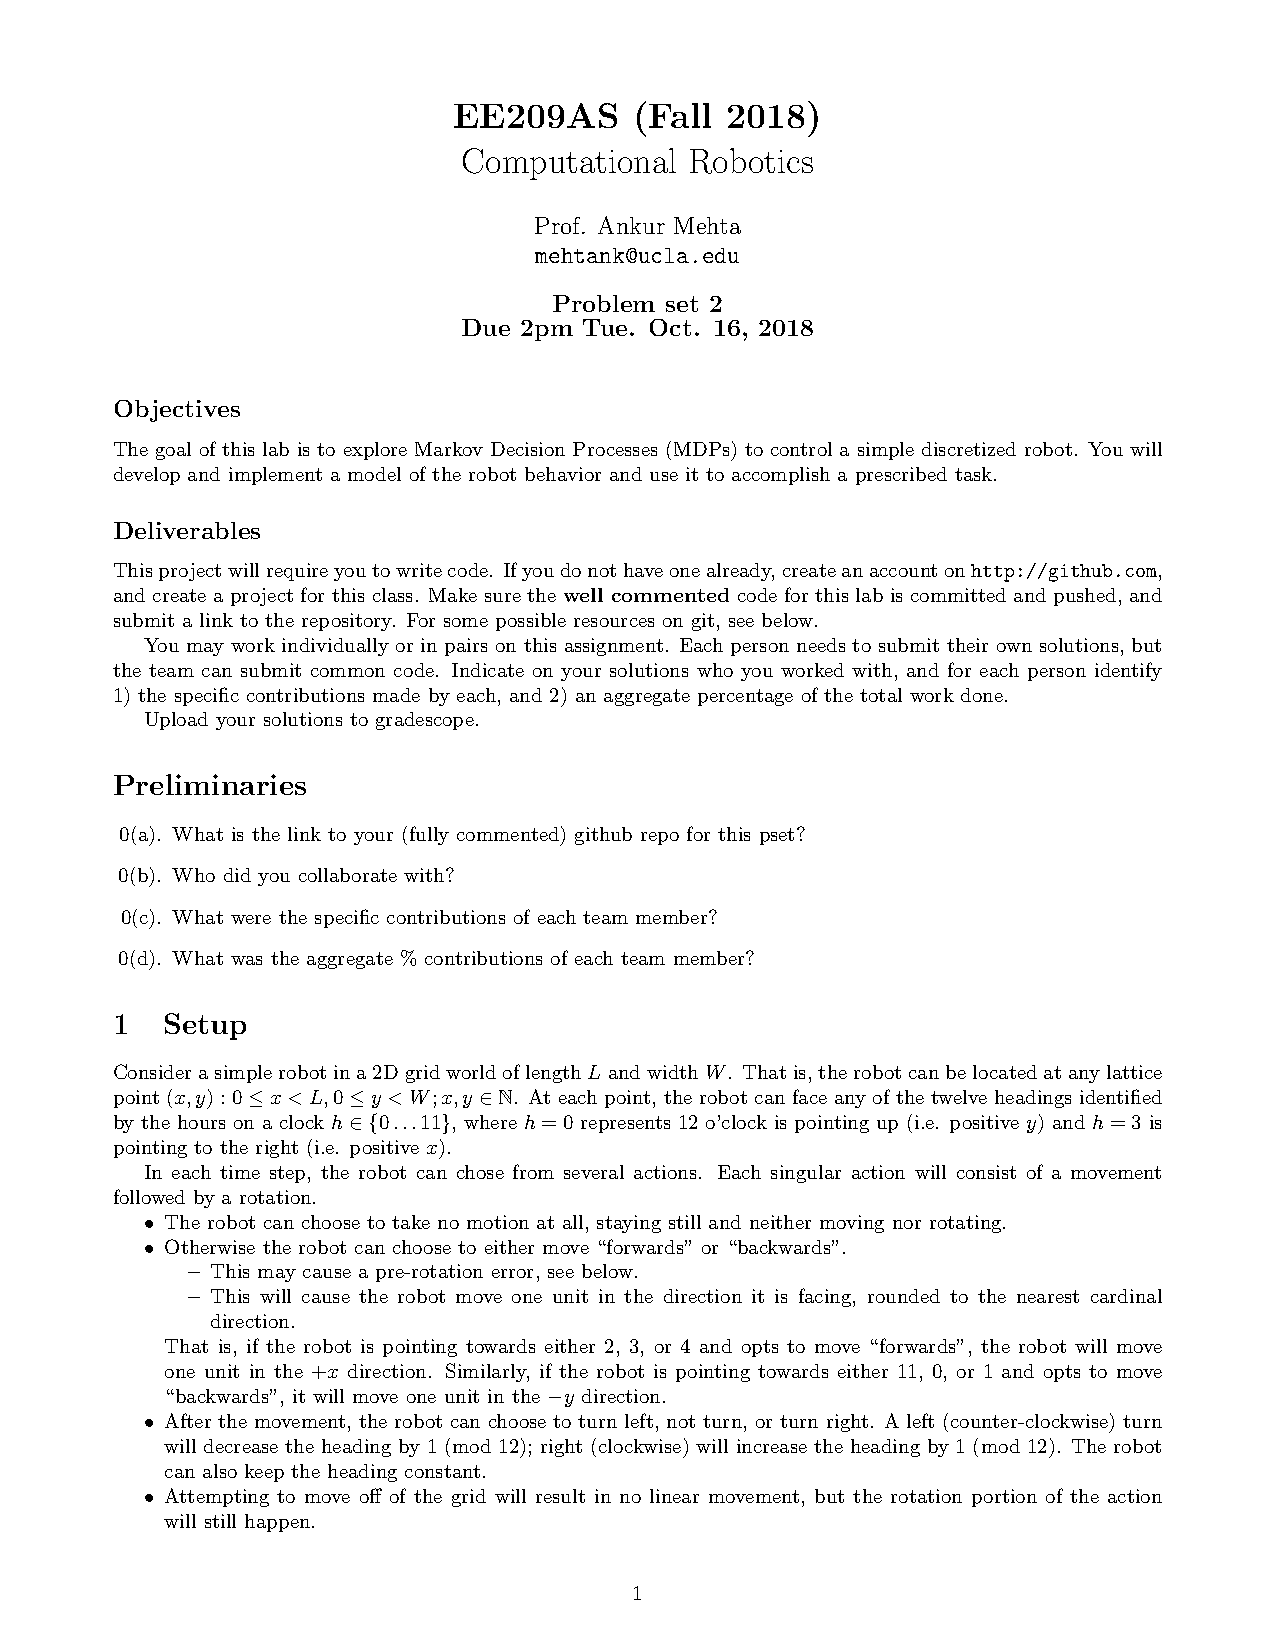
\includepdf[pages={1-}]{pset2.pdf}  % to include all pages
	
	\begin{center}
	
	\LARGE Name: Sahba Aghajani Pedram \\
	\LARGE UID: 504616252 \\
	\LARGE Email: sahbaap@ucla.edu \\
	
	\vspace{30pt}
	\textbf{Problem Set 2} \\
 	Due 2pm Thursday Oct. 18, 2018 
 	
	 \end{center}

	\vspace{30pt}

	\section*{Preliminaries}
	\noindent 0(a) \url{https://github.com/Sahbaap/ComputationalRoboticsUCLAEE209}          \\ \\ \\
	\noindent 0(b) I did all by myself. \\ \\ \\
	\noindent 0(c) 100\% myself. \\ \\ \\
	\noindent 0(d) 100\% myself. \\ \\ \\
	
	
	
	\newpage
	\section*{1  Setup}
	\noindent 1(a) The state of the robot is composed of a tuple $(x,y,h)$ where $0 \le x < L$ , $0 \le y < W$, and $0 \le h \le 11$ and $x,y,h \in \mathbb{N}$. So the size of the state space is $N_{s} = L \times W \times 12$. \\
	Note that I have defined the state class where I can instantiate the state of the robot with any (x,y,h). Moreover, I have define the environment class where I can instantiate the maze with given L and W. 
	
	\section*{State Space}
	\lstinputlisting{create_statespace.m} \vspace{30pt}
	\section*{State Class}
	\lstinputlisting{state.m} \vspace{30pt}
	\section*{Environment Class}
	\lstinputlisting{environment.m} \vspace{30pt}
	
	\noindent 1(b) The size of the action space is $N_{a} = 7$. At each time step, the robot can (1) stay and not move, (2) move forward and turn right, (3) move forward and turn left, (4) move forward and not turn, (5) move backward and turn left, (6) move backward and turn right, and (7) move backward and not turn.
	\section*{Action Class}
	\lstinputlisting{action.m} \vspace{30pt}
	
	\newpage
	\noindent 1(c)
	\section*{Transition Probability}
	\lstinputlisting{Transition_Probability.m} \vspace{30pt}
	
	\newpage
	\noindent 1(d)
	\section*{Dynamics}
	\lstinputlisting{f.m}
	
	\newpage
	\section*{2  Problem}

	\noindent 2(a)
	\section*{Reward}
	\lstinputlisting{reward.m}
	
	\newpage
	\section*{3  Policy iteration}
	\noindent 3(a)
	\section*{Generating initial policy $\pi_{0}$}
	\lstinputlisting{generate_policy.m}
	\lstinputlisting{state_to_goal_relative.m}
	\newpage
	\lstinputlisting{generate_initial_policy.m}
	
	\newpage
	\noindent 3(b)
	\section*{Trajectory plot}
	\lstinputlisting{generate_plot_trajectory.m}
	
	\newpage
	\noindent 3(c) 
	\section*{Trajectory starting at (1,4,6)}
	The following sequence of actions were taken to move the robot from (1,4,6) tuple to the goal with (3,5,-) where only x and y positions of the goal matter. Fig. 1 shows the robot's trajectory under initial policy \\
	
	\noindent1- Move Forward, Turn left   \hspace{20pt}    2- Move Forward, Turn left \hspace{20pt}    3- Move Forward, Turn left \\ 
	4- Move Forward, Turn left   \hspace{20pt}    5- Move Forward, Turn left \hspace{20pt}    6- Move Forward, Turn left \\
	7- Move Forward, Turn left   \hspace{20pt}    8- Move Forward, Turn left \hspace{20pt}    9- Move Forward, Turn left \\
	10- Move Forward, Turn left   \hspace{20pt}    11- Move Backward, Turn left \hspace{20pt}    12- Move Forward, No Turn
	
	\begin{figure}[h!]
		\centering
		\includegraphics[trim={5cm 9cm 5cm 5cm},clip,scale = 1]{plots/PolicyIteration/3c.pdf}
		\caption{Robot's trajectory starting at state (1,4,6) under initial policy.}
	\end{figure}

	\newpage
	\noindent 3(d) 	
	\section*{Policy evaluation}
	\lstinputlisting{evaluate_policy.m}
	
	\newpage
	\noindent 3(e) 
	\section*{Evaluation of initial policy $\pi_{0}$}
	The value of the trajectory in 3(c) is -77.36. A plot of V values across the grid with robot's heading (h) be equal to 6, i.e. robot is pointing down, is shown in Fig. 2. Of note, it is expected that the final value of V at goal should be $\frac{1}{1-0.9} = 10$ at infinity time limit which it is.
	
	\begin{figure}[h!]
		\centering
		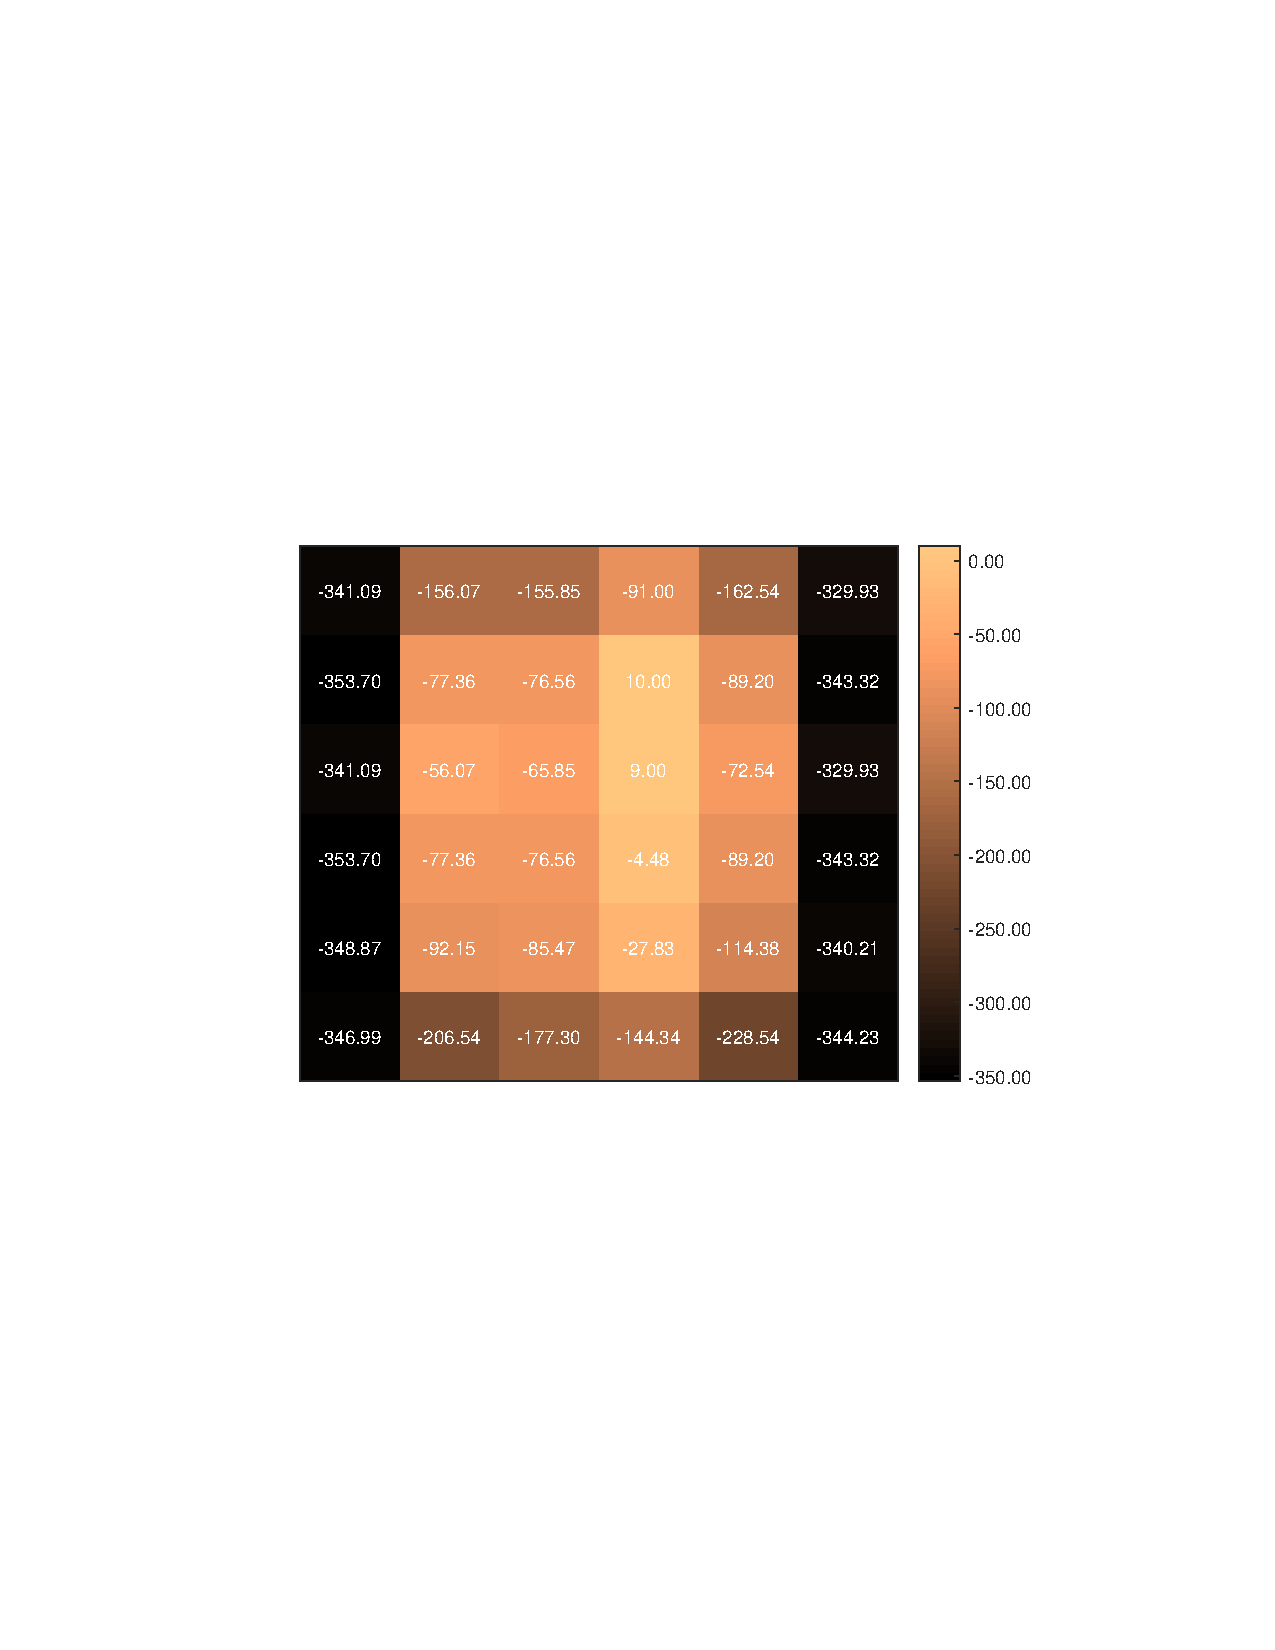
\includegraphics[trim={5cm 9cm 3cm 5cm},clip,scale = 1]{plots/PolicyIteration/3e.pdf}
		\caption{V values of different robot's states (heading = 6) under initial policy.}
	\end{figure}

	\newpage
	\noindent 3(f) 	
	\section*{Policy update}
	\lstinputlisting{update_policy.m}

	\newpage
	\noindent 3(g) 	
	\section*{Policy iteration}
	\lstinputlisting{policy_iteration.m}

	\newpage
	\noindent 3(h)
	\section*{Optimal robot trajectory and value starting at (1,4,6) under $P^*$ and $V^*$}
	Under this optimal policy, the $V^*$ of the robot at state (1,4,6) is 3.48. Note that the heat of V is for robot states whose headings are 6.	The $\pi^{*}$ of the robot is: \\
	
	\noindent1- Move Forward, Turn left   \hspace{20pt}    2- Move Forward, No Turn \hspace{20pt}    3- Move Forward, Turn left \\ 
	4- Move Forward, No Turn  \hspace{20pt}    5- Move Forward, Turn right \hspace{20pt}    6- Move Backward, No Turn \\
	7- Move Backward, No Turn   \hspace{20pt}    8- Move Backward, Turn left
	
	\vspace{50pt}  
	\begin{figure}[h!]
\centering
\begin{minipage}{0.5\textwidth}%
	\subfloat[Subfigure 2 list of figures text][Optimal Policy ($P^*$) obtained from policy iteration algorithm.]{
		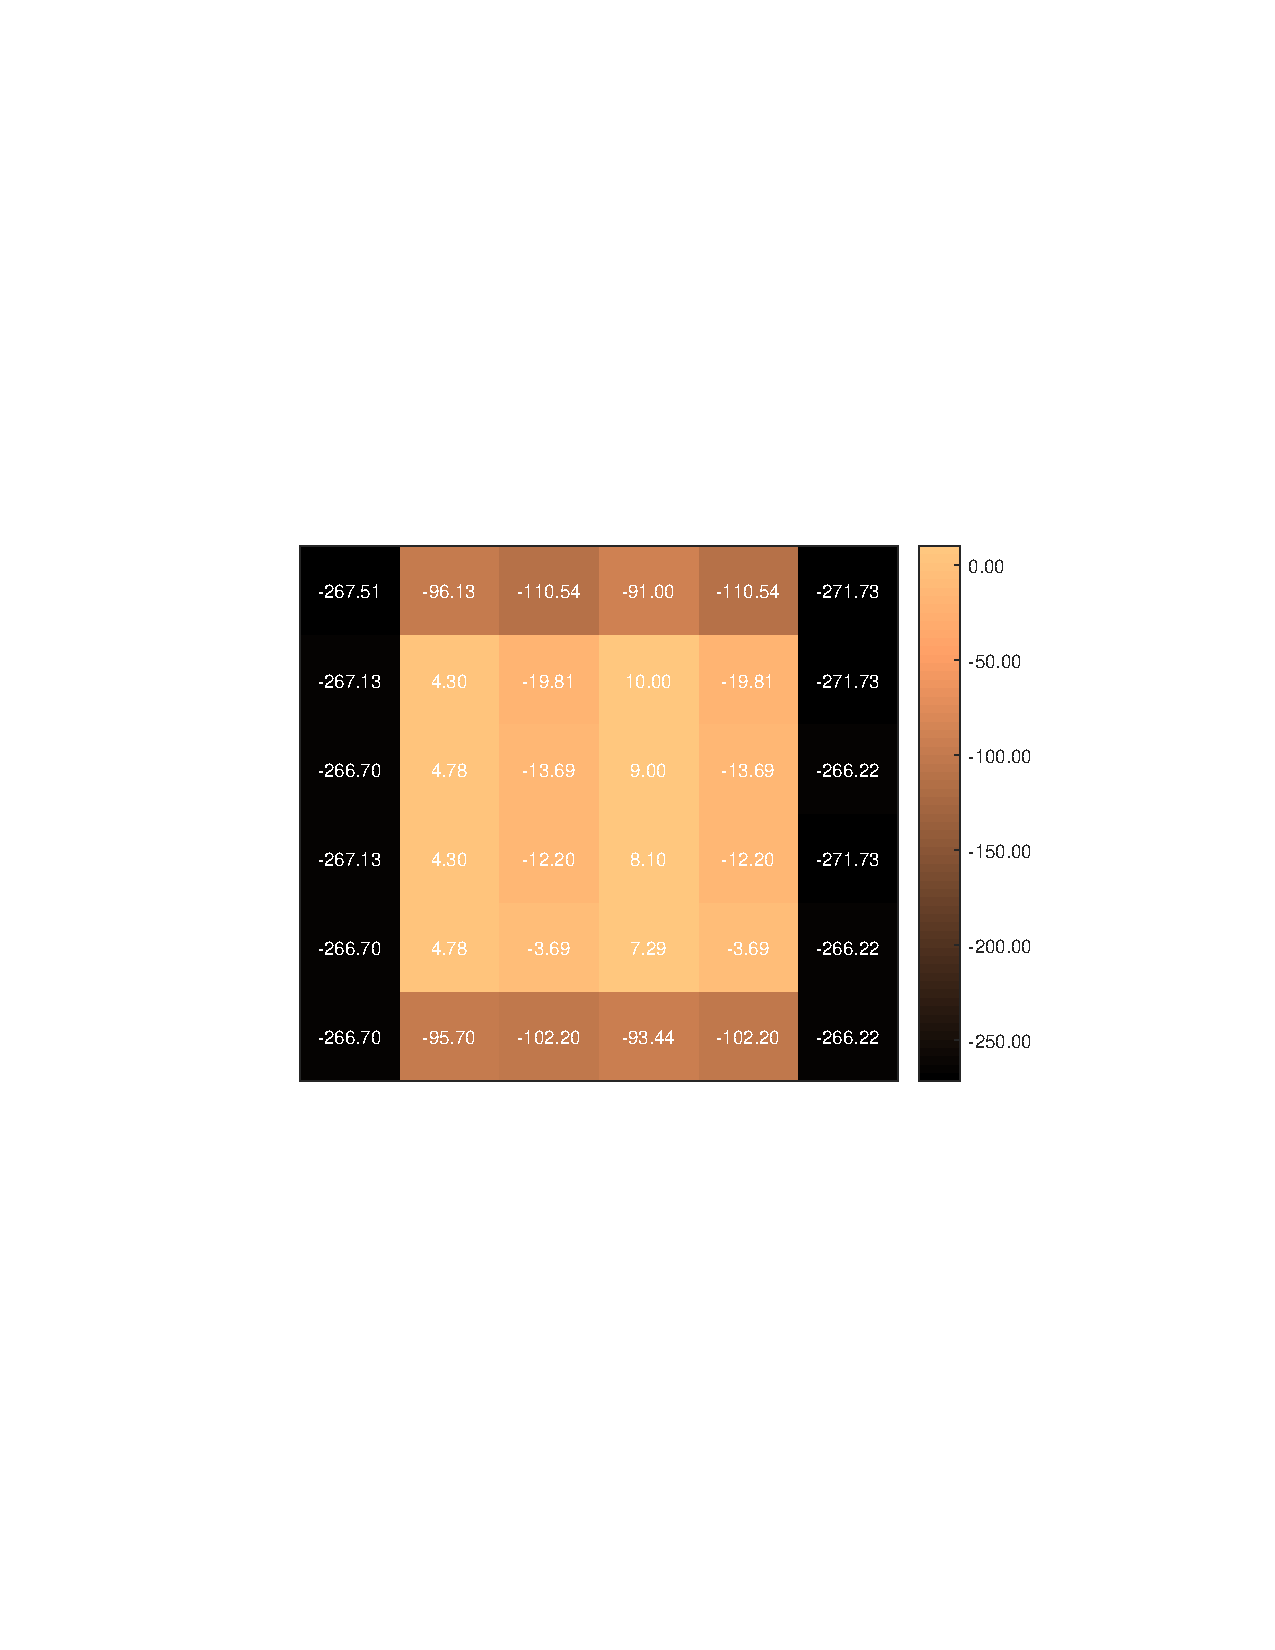
\includegraphics[trim={5cm 9cm 3cm 9cm},clip,scale = 0.7]{plots/PolicyIteration/3h1.pdf}
		\label{fig:subfig2}} 
\end{minipage}
\qquad
\begin{minipage}{0.4\textwidth}%
	\subfloat[Subfigure 2 list of figures text][Optimal Value ($V^*$) obtained from policy iteration algorithm.]{
		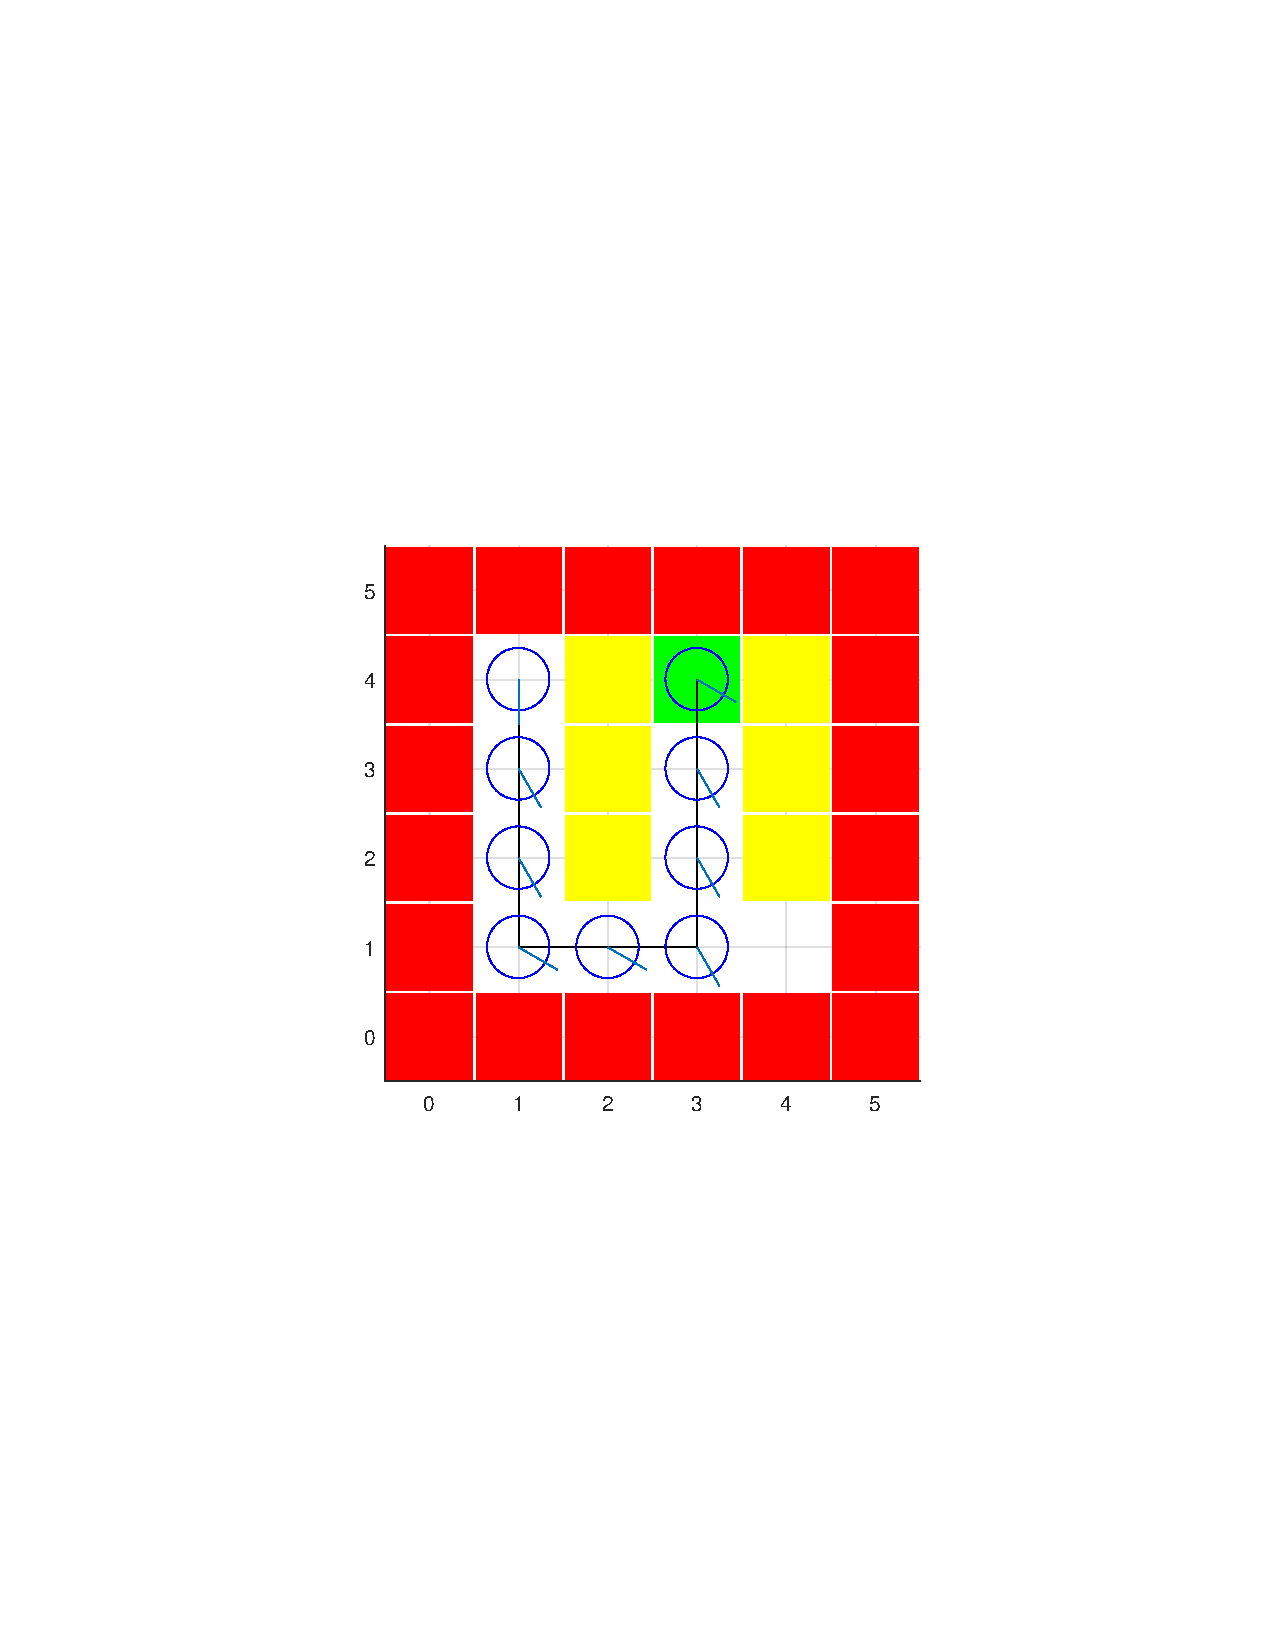
\includegraphics[trim={5cm 9cm 3cm 9cm},clip,scale = 0.7]{plots/PolicyIteration/3h2.pdf}
		\label{fig:subfig2}} 
\end{minipage}

\caption{Question 3(h).}
\label{fig:globfig}
\end{figure}	

	
	
	\newpage
	\noindent 3(i) 	On my Lenovo ThinkPad laptop with 64-bit windows 10, 2.5 GHz CPU and 8 GB RAM, it took 272 (s) for policy iteration to run. 
	
	%\includepdf{3c.pdf}
	%\includepdf[pages=-]{3c.pdf}
	
	\newpage
	\section*{4  Value iteration}
	\noindent 4(a) 	
	\section*{Value iteration}
	\lstinputlisting{value_iteration.m}
	
	\newpage
	\noindent 4(b) 	
	The $V^*$ for this policy with initial $s_{0}$ at (1,4,6) is 4.30 -- see Fig. 4. As it can be seen, both value iteration and policy iteration algorithms yield to identical results for both $V^*$ but with slightly different $\pi^{*}$. This is totally expected as both methods solved the same underlying Bellman equation for $V^*$. The optimal policy, as it happened here, is not unique however. This means that several optimal policies can result in the same optimal value function.\\
	Note that the computational complexity of both methods is also $N_{A}*N_{S}^2$. But since they have slightly different approaches, sometimes one converges faster than the other and vice versa. In fact the constant that multiplies to this complexity is different. \\
	
	\noindent The optimal policy in this case is:
	
	\noindent1- Move Forward, Turn left   \hspace{20pt}    2- Move Forward, No Turn \hspace{20pt}    3- Move Forward, Turn left \\ 
	4- Move Forward, No Turn  \hspace{20pt}    5- Move Forward, Turn right \hspace{20pt}    6- Move Backward, Turn right. \\
	7- Move Backward, Turn left  \hspace{20pt}  8- Move Backward, Turn left
	
	\vspace{50pt}  
	\begin{figure}[h!]
		\centering
		\begin{minipage}{0.5\textwidth}%
			\subfloat[Subfigure 2 list of figures text][Optimal Policy ($P^*$) obtained from value iteration algorithm.]{
				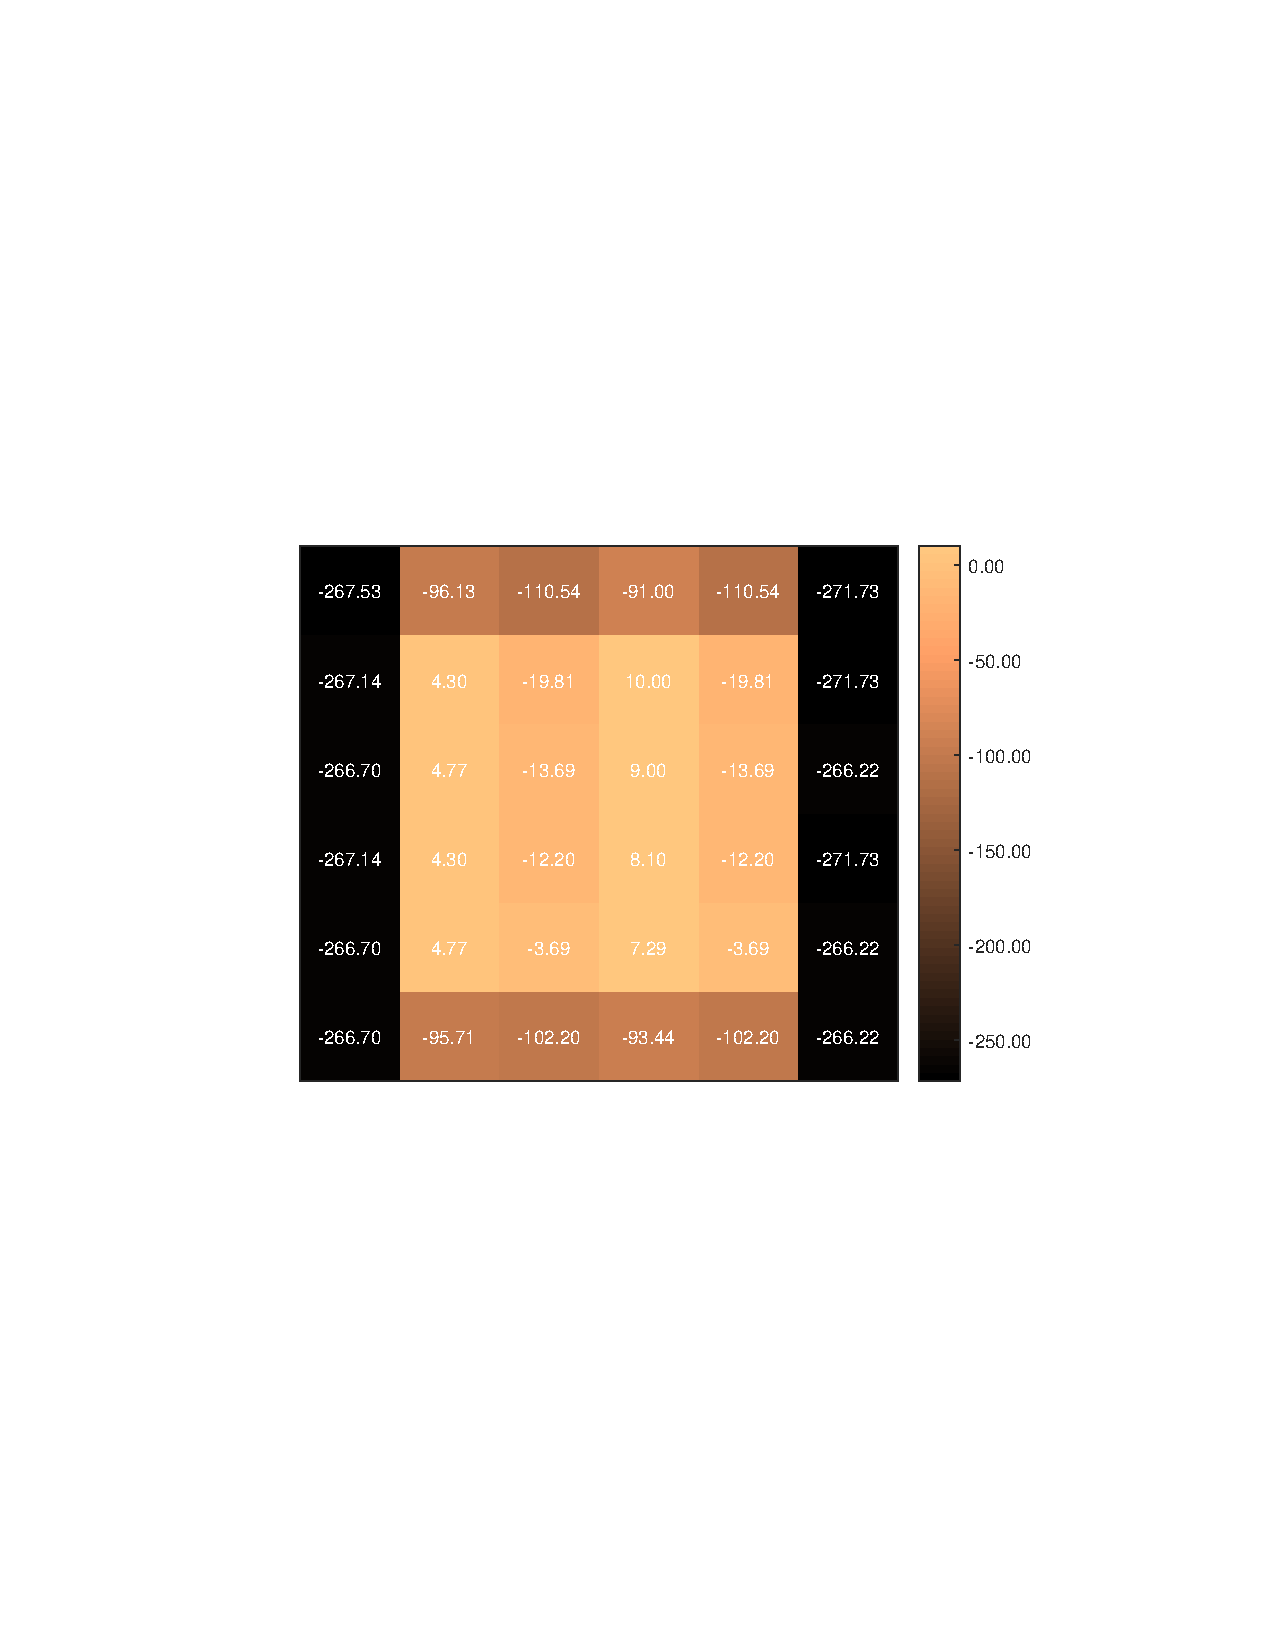
\includegraphics[trim={5cm 9cm 3cm 9cm},clip,scale = 0.7]{plots/ValueIteration/4b1.pdf}
				\label{fig:subfig2}} 
		\end{minipage}
		\qquad
		\begin{minipage}{0.4\textwidth}%
			\subfloat[Subfigure 2 list of figures text][Optimal Policy ($P^*$) obtained from value iteration algorithm.]{
				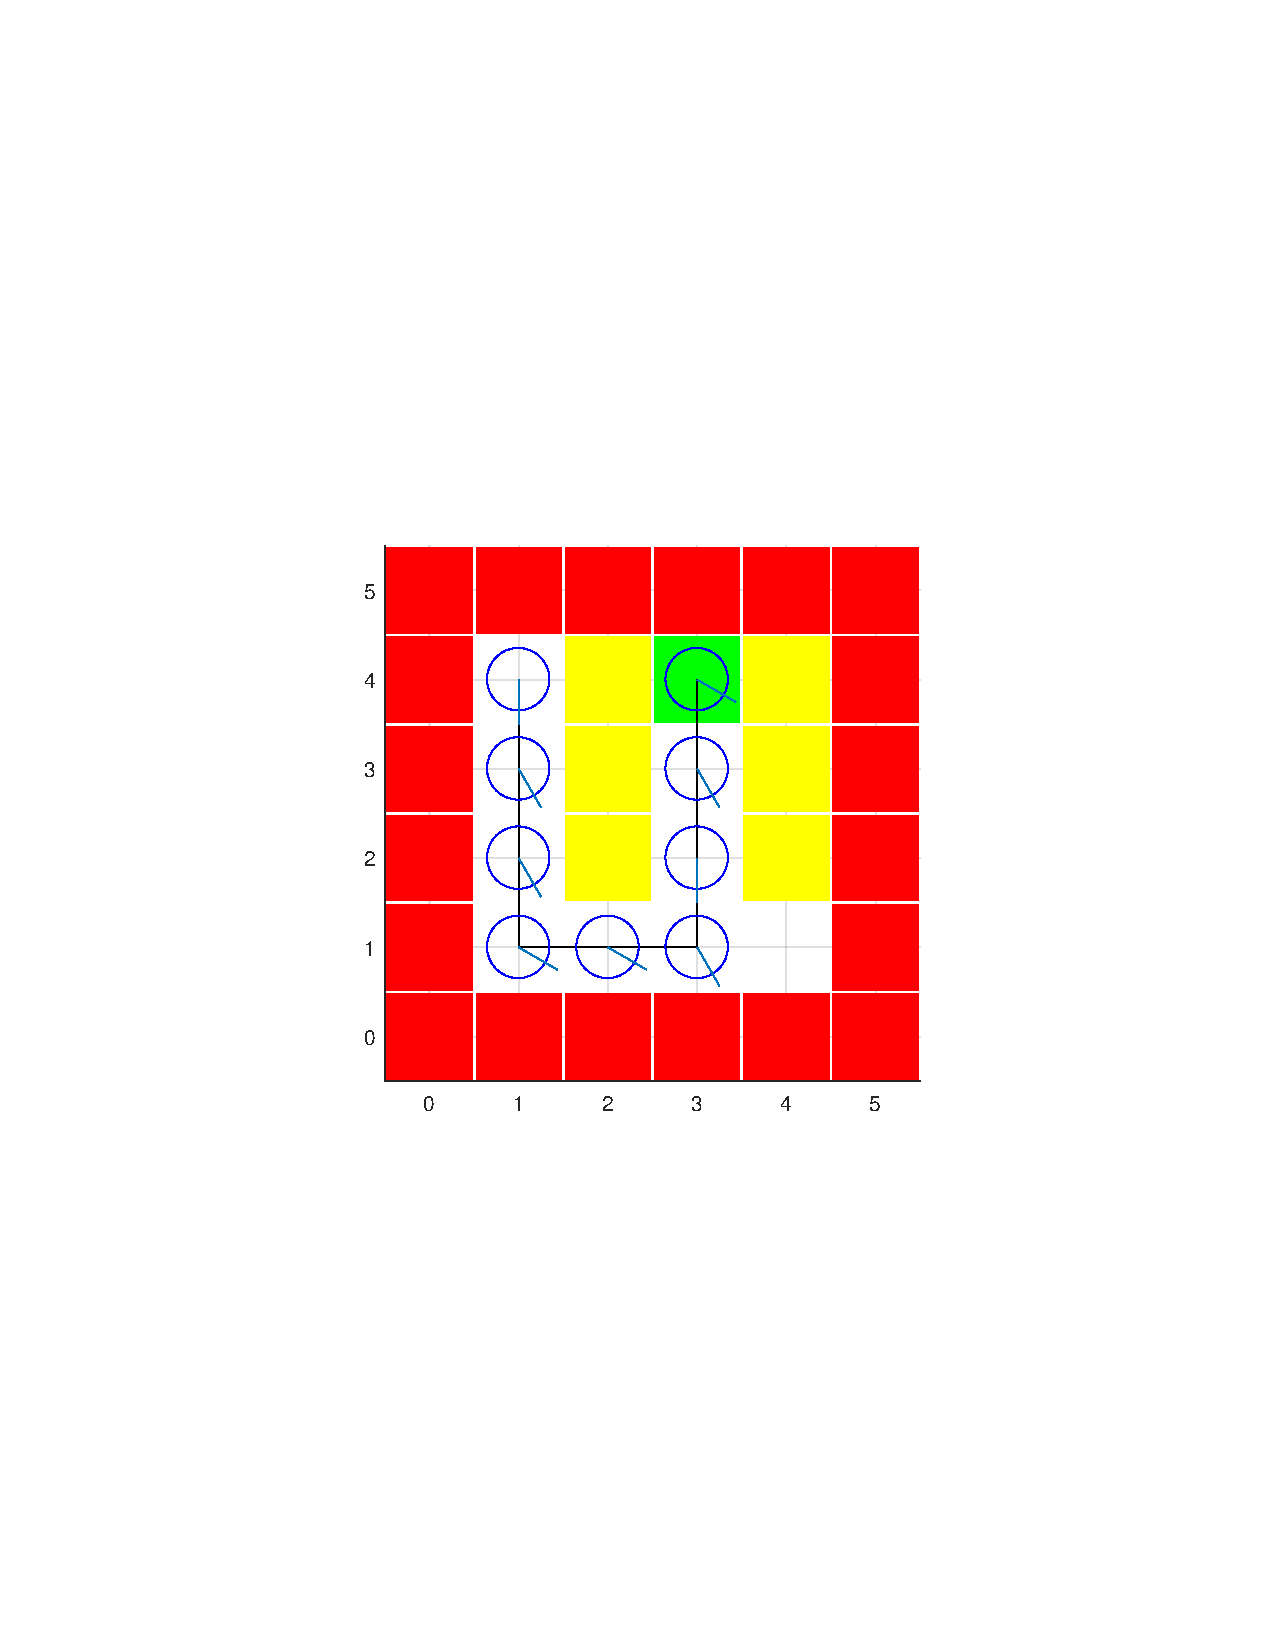
\includegraphics[trim={5cm 9cm 3cm 9cm},clip,scale = 0.7]{plots/ValueIteration/4b2.pdf}
				\label{fig:subfig2}} 
		\end{minipage}
		
		\caption{Question 4(b).}
		\label{fig:globfig}
	\end{figure}	
	
	\newpage
	\noindent 4(c) 	
	On my Lenovo ThinkPad laptop with 64-bit windows 10, 2.5 GHz CPU and 8 GB RAM, it took 571 (s) for this value iteration to run. As it can be seen the value iteration took more than two times to converge compared to the policy iteration. 

	\newpage
	\section*{5  Additional scenarios}
	\noindent 5(a)
	 	With $P_{e} = 0.25$, The optimal expected V ($V^*$) for the robot at state (1,4,6) os -6.86. Note that this means that if we run, for example, a Monte Carlo simulation and average the V values under this optimal policy starting at (1,4,6), this averaged V value will be -6.86. However, each time we run the simulation we are going to get V values that are different than -6.86 and their average will eventually converge to -6.86. \\
		In terms of actions also, note that the robot's trajectory changes for every realization of the policy. This means that every time we run our matlab program it gives us different robot trajectory due to the pre-rotation error in our robot which is expressed in $P_{e}$. \\
		I have included a plot of expected V values across robot states with heading equal to 6 (see Fig. 5). At the same time I have included different realizations of robot trajectory along with the value of that specific trajectory under the optimal policy.
\vspace{50pt}  
\begin{figure}[h!]
	\centering
	\begin{minipage}{0.5\textwidth}%
		\subfloat[Subfigure 2 list of figures text][Expected Optimal Value ($V^*$) under $P_{e} = 0.25$]{
			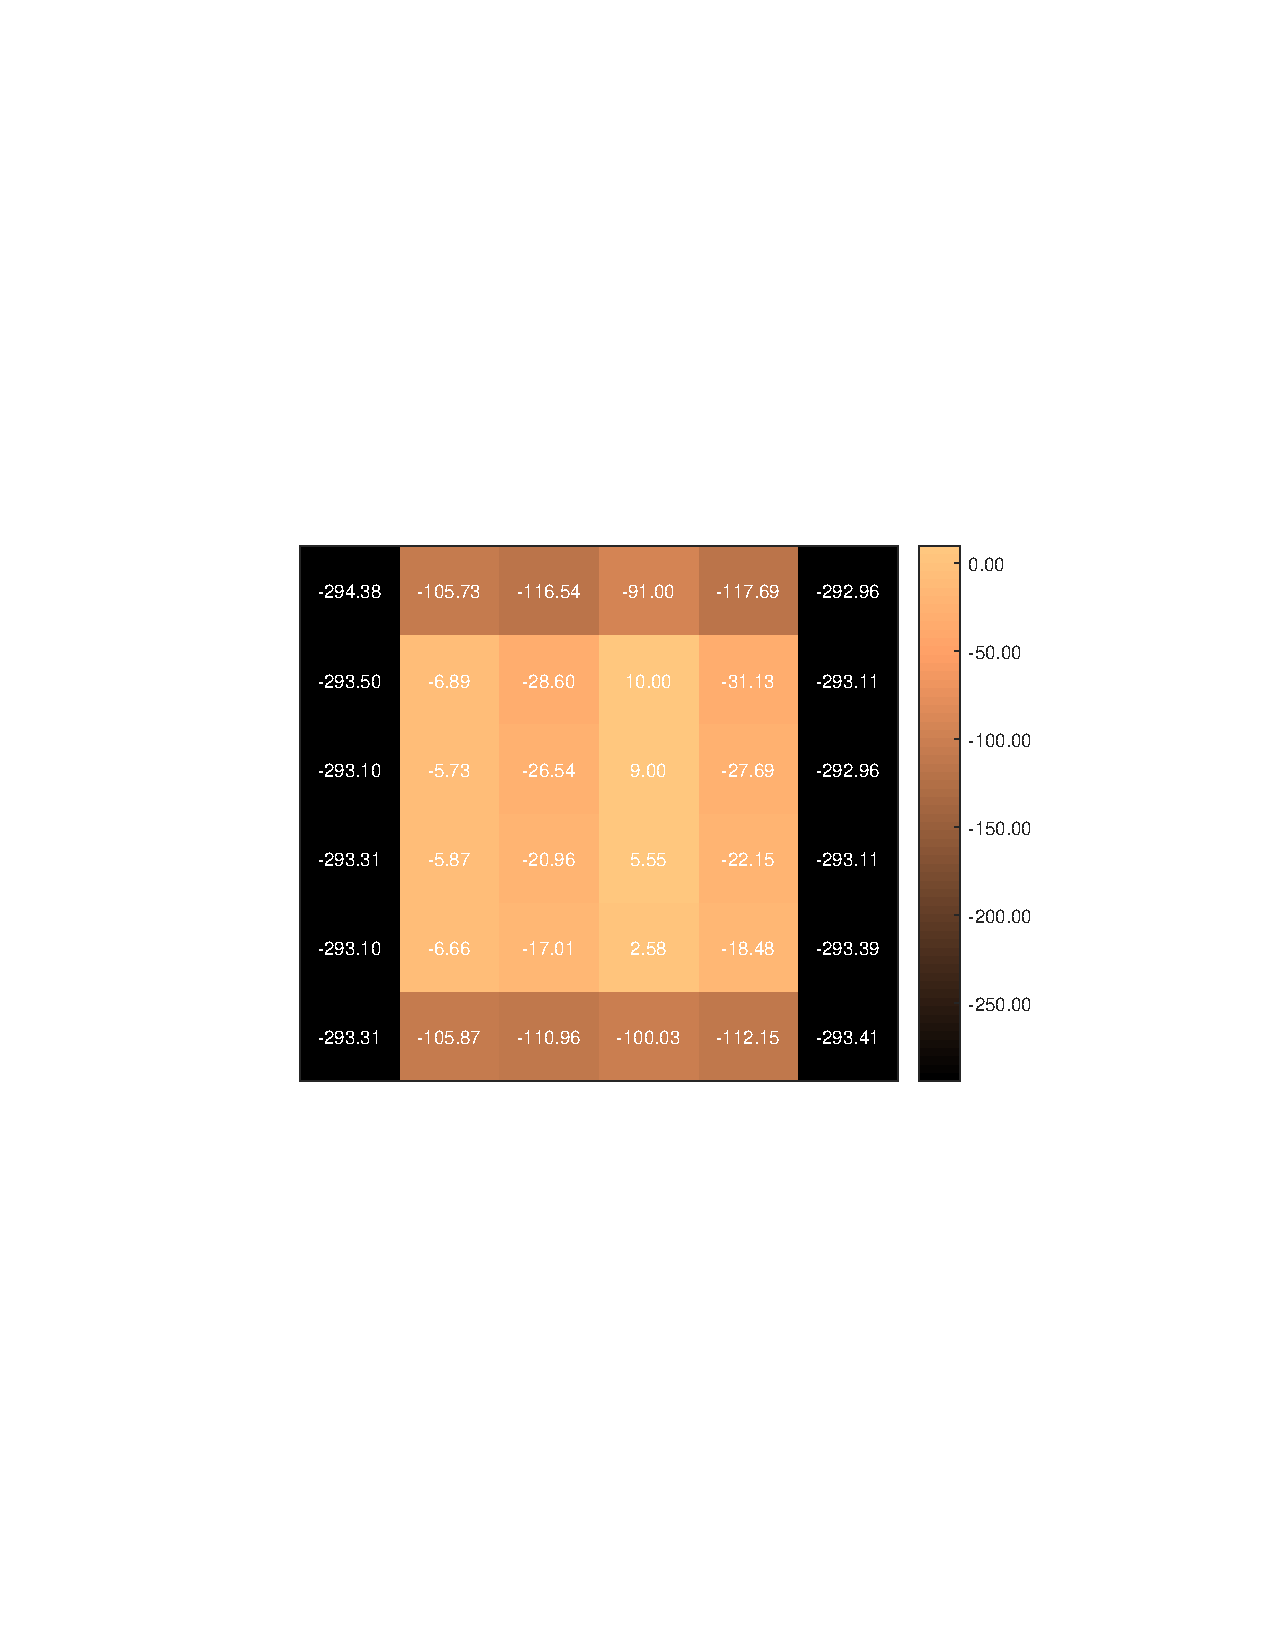
\includegraphics[trim={5cm 9cm 3cm 9cm},clip,scale = 0.55]{plots/Probabilistic/5a1.pdf}
			\label{fig:subfig2}} \\
		
			\subfloat[Subfigure 3 list of figures text][$V_{1}$ with value of -14.86]{
			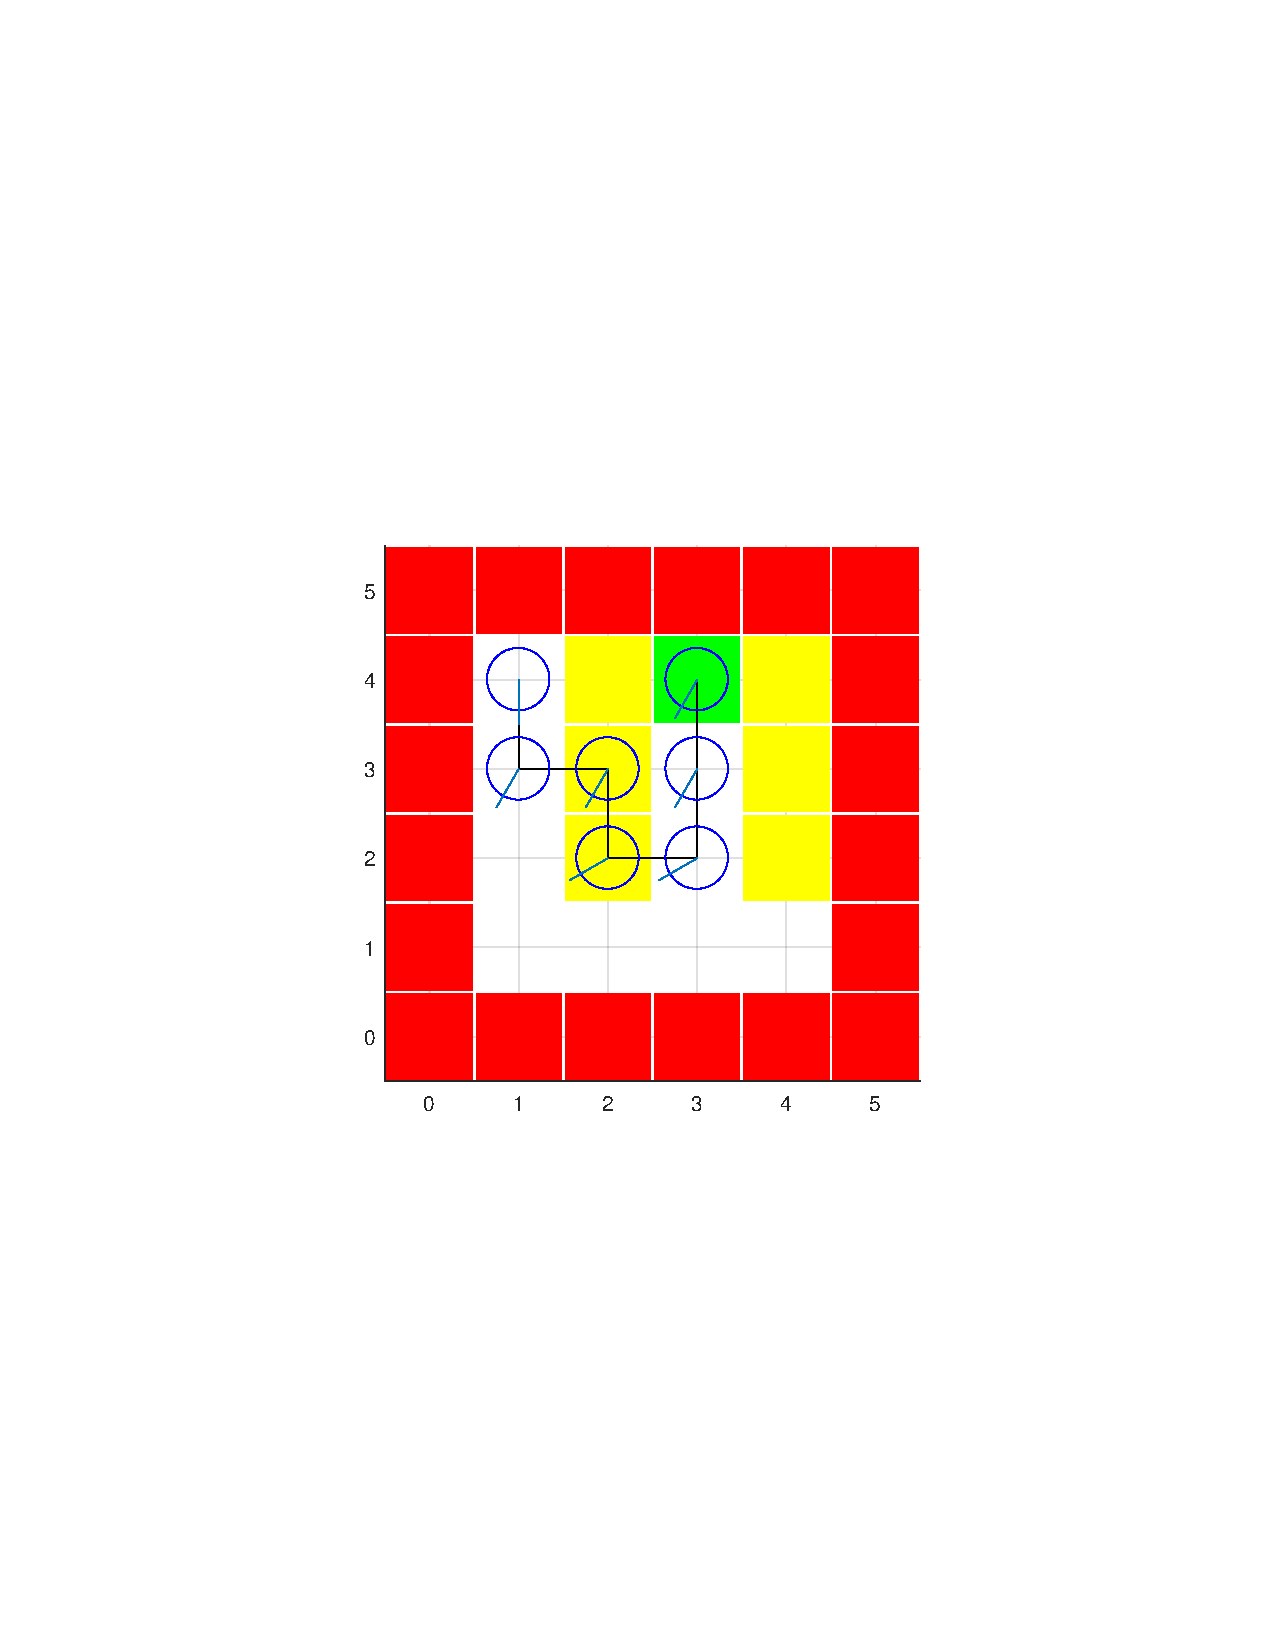
\includegraphics[trim={5cm 9cm 3cm 9cm},clip,scale = 0.55]{plots/Probabilistic/5a2.pdf}
			\label{fig:subfig2}} \\
		
			\subfloat[Subfigure 3 list of figures text][$V_{2}$ with value of -10.34]{
			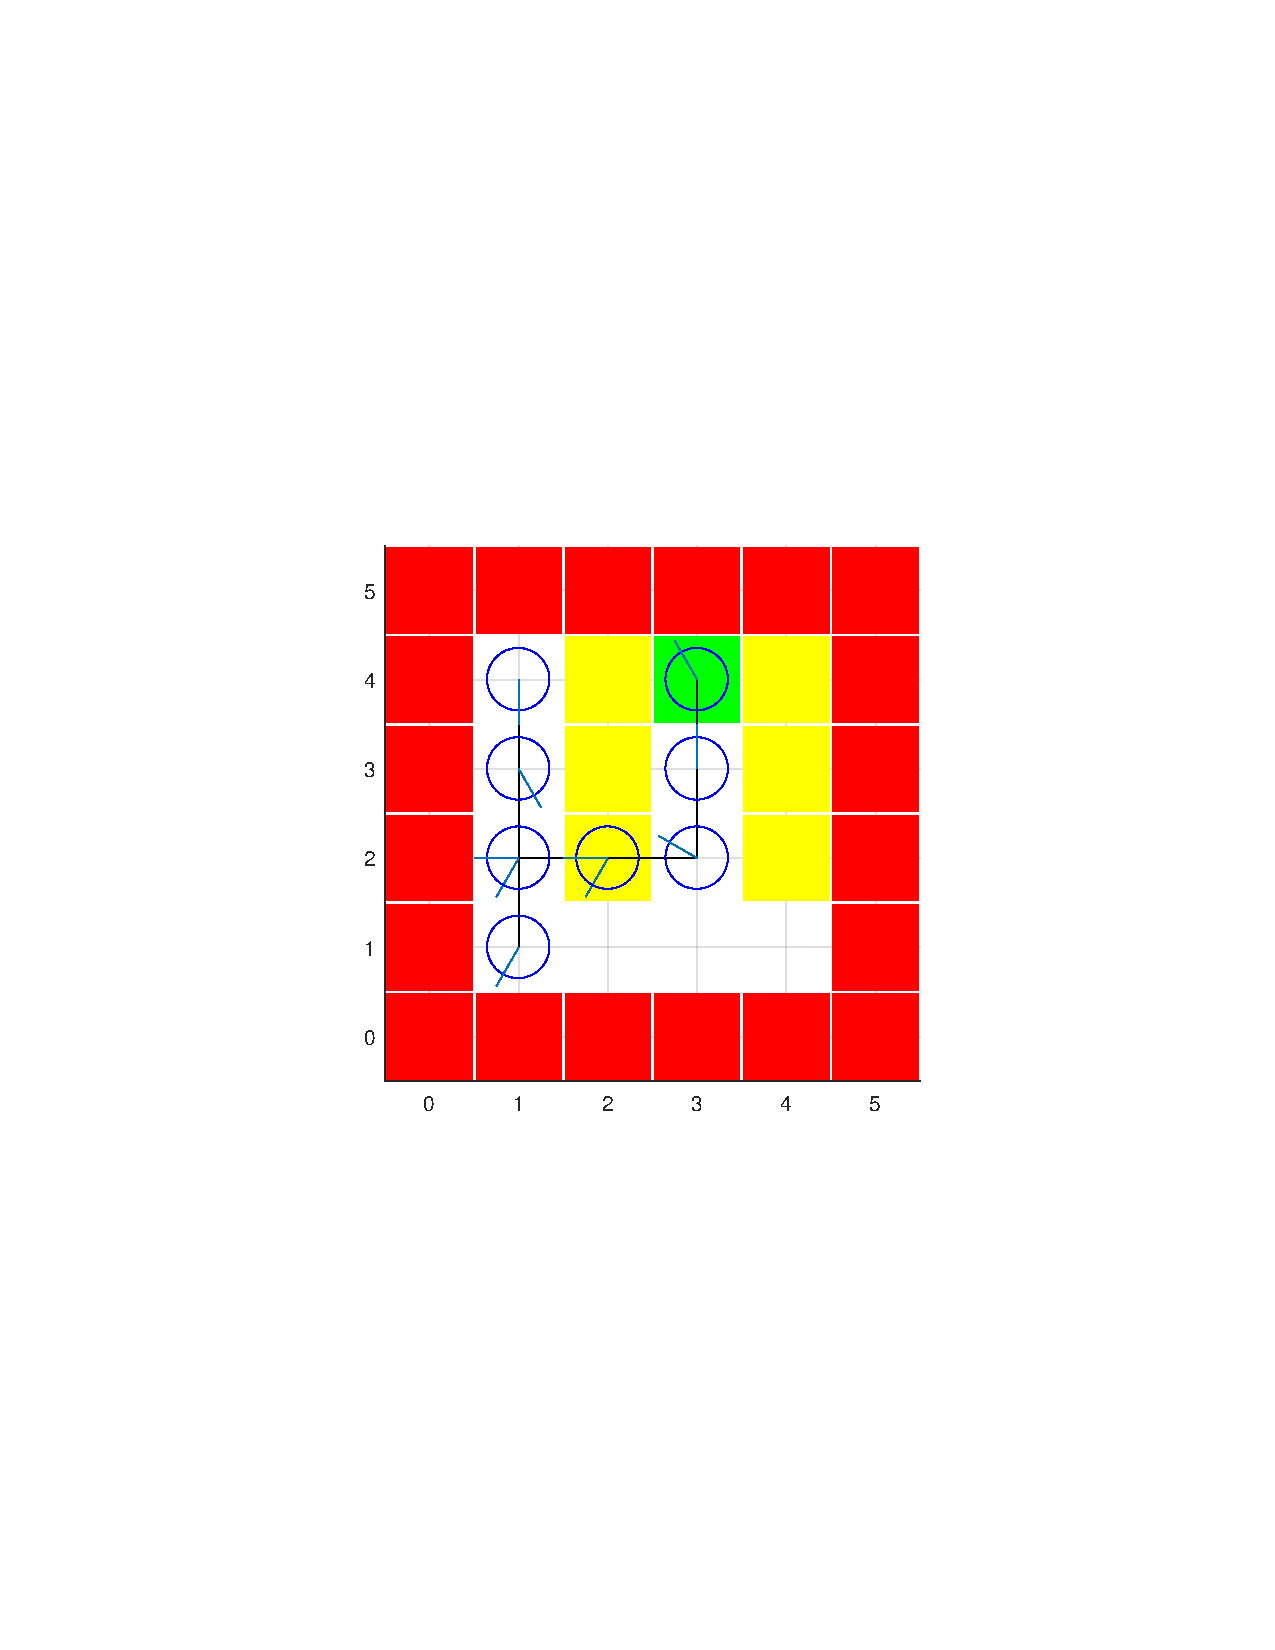
\includegraphics[trim={5cm 9cm 3cm 9cm},clip,scale = 0.55]{plots/Probabilistic/5a21.pdf}
			\label{fig:subfig2}} 
	\end{minipage}
	\qquad
	\begin{minipage}{0.4\textwidth}%
		\subfloat[Subfigure 2 list of figures text][$V_{3}$ with value of -8.37]{
			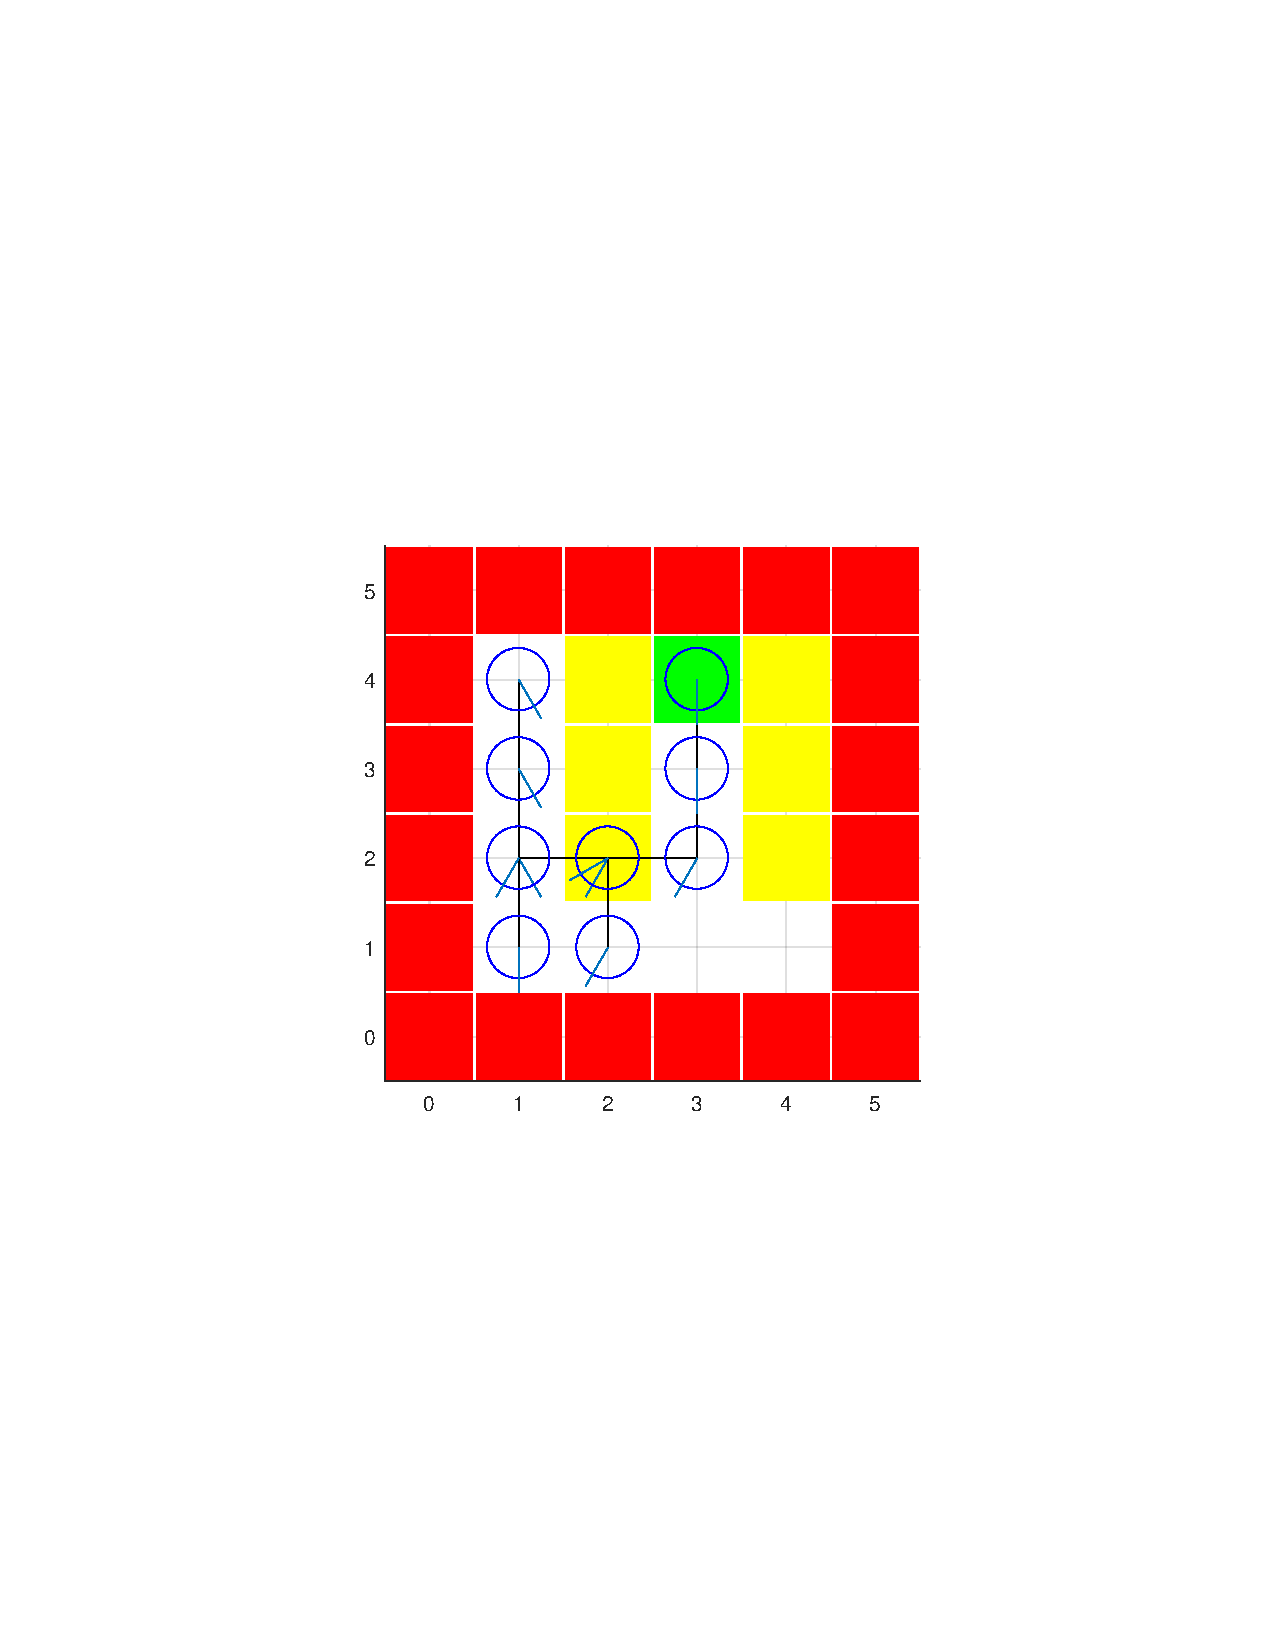
\includegraphics[trim={5cm 9cm 3cm 9cm},clip,scale = 0.55]{plots/Probabilistic/5a22.pdf}
			\label{fig:subfig2}} 
		
			\subfloat[Subfigure 3 list of figures text][$V_{4}$ with value of -3.52]{
			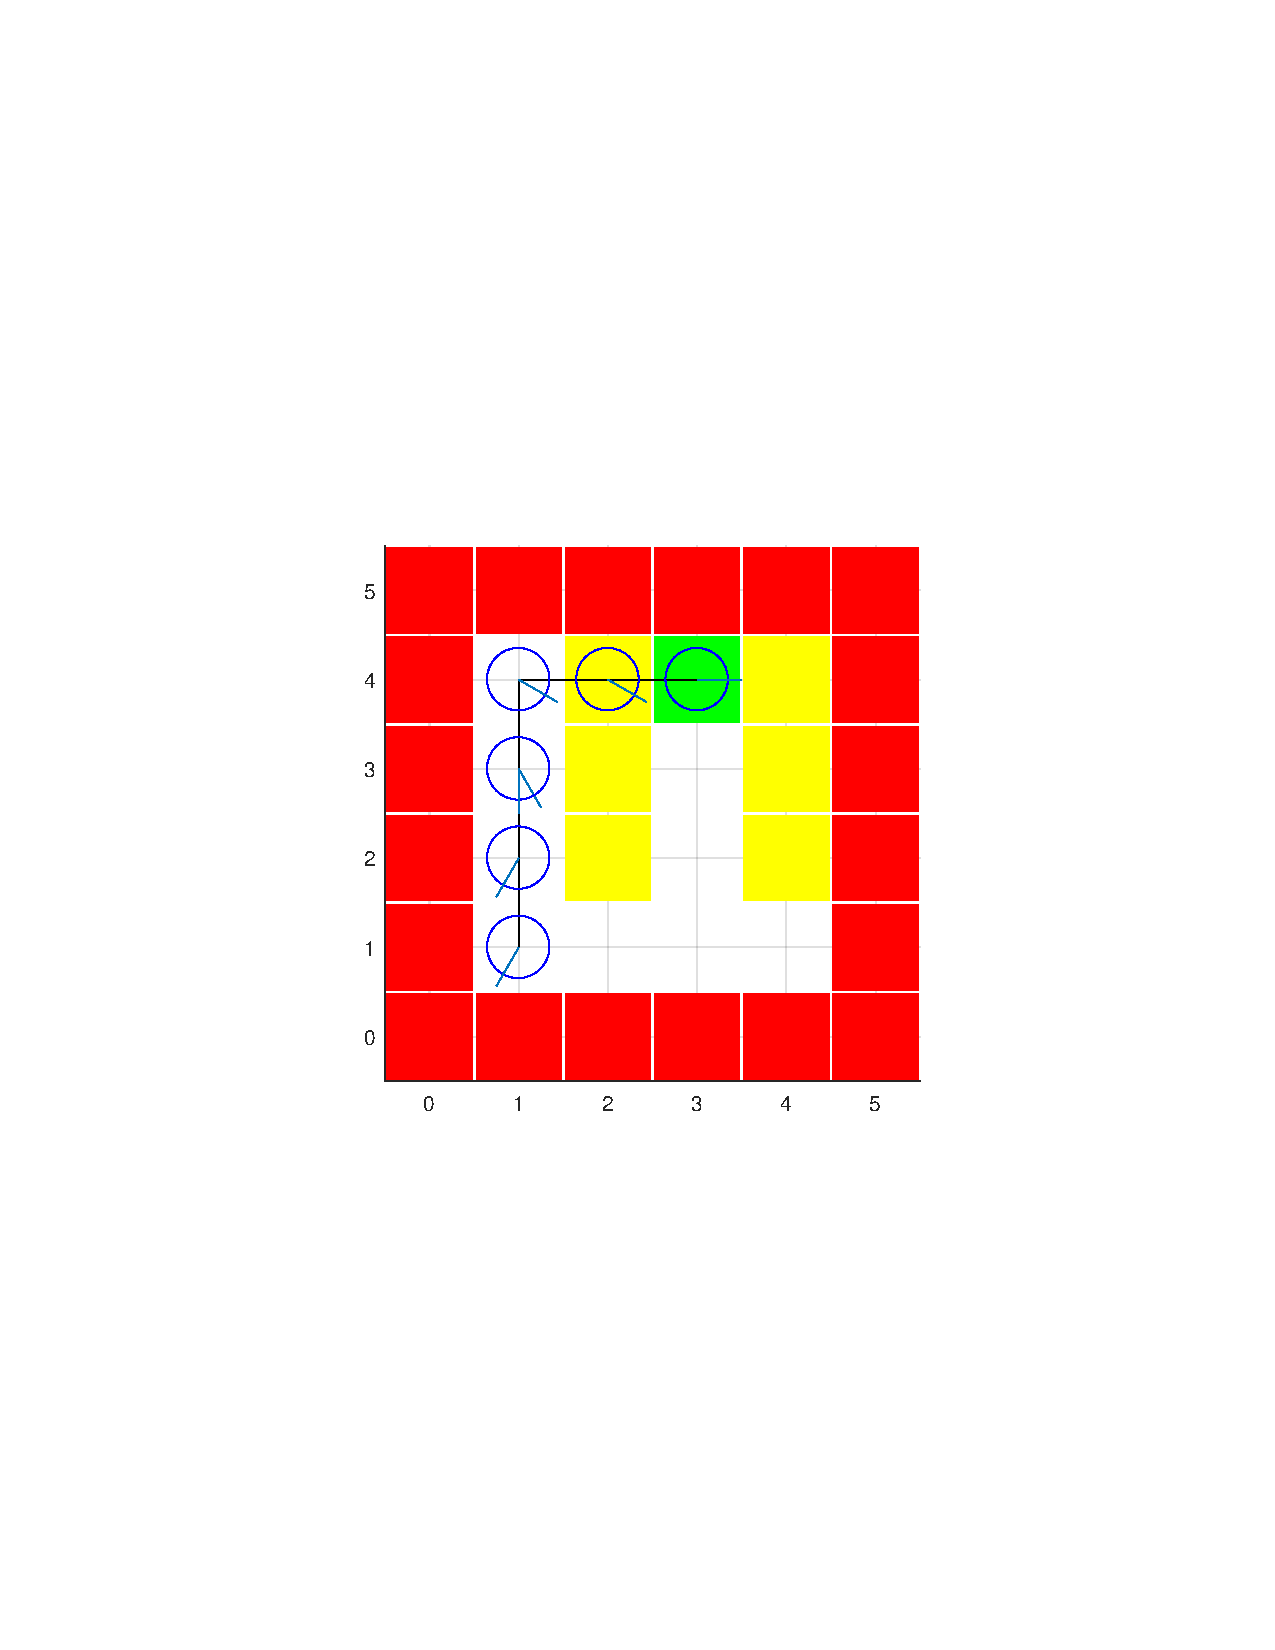
\includegraphics[trim={5cm 9cm 3cm 9cm},clip,scale = 0.55]{plots/Probabilistic/5a23.pdf}
			\label{fig:subfig3}} \\ 
		
			\subfloat[Subfigure 3 list of figures text][$V_{5}$ with value of -4.97]{
			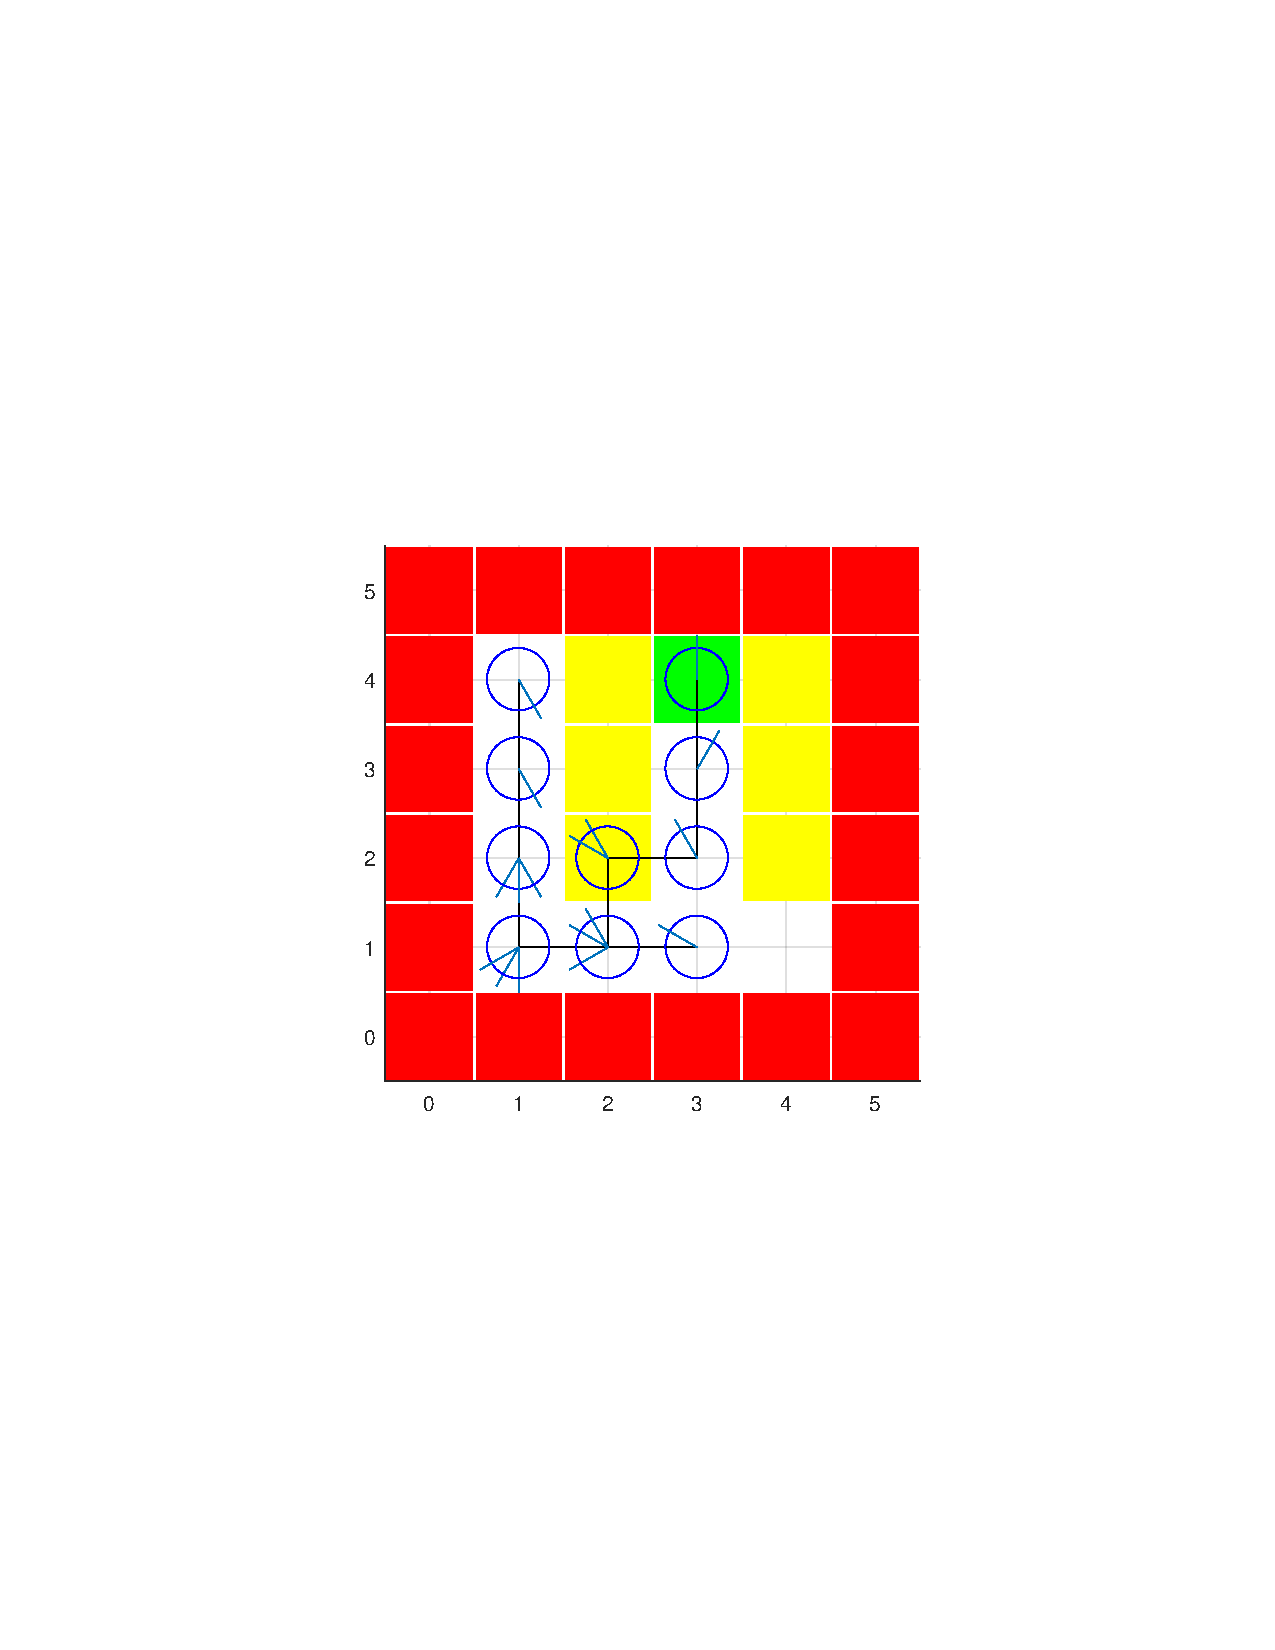
\includegraphics[trim={5cm 9cm 3cm 9cm},clip,scale = 0.55]{plots/Probabilistic/5a24.pdf}
			\label{fig:subfig3}} 
	\end{minipage}
	
	\caption{Question 5(a).}
	\label{fig:globfig}
\end{figure}	
	
	\newpage
	\newpage
	\noindent 5(b) 	
	In this section, the robot only gets the final reward with specific headings (5,6,7) rather than all headings. Since the final robot state in previous sections under optimal policy was in the heading 5, when I ran the value iteration or policy iteration algorithms, the same optimal policy and value for the robot at (1,4,6) is obtained (as it can be seen in the Figures.). In this case in took 705 (s) for the value iteration algorithm to converge while it took 422 (s) for the policy iteration to converge. Again value iteration and policy suggests two slightly different trajectories for robot to follow starting at (1,4,6). Fig. 6 and Fig. 7 show these plots. 
	
	\newpage
	When $P_{e} = 0.25$, $V^*$ and $P^*$ change compared to the case where the heading of the robot did not matter at goal point of (3,4). Fig 8 shows the V map at robot heading of 6 and as it can be seen, the $V^*$ of point (1,4,6) which is the expected value of sum of the discounted rewards is -8.30 as opposed to the other case (problem 5a) which was -6.89. In this case it took 798 (s) for the value iteration algorithm to converge and 400 (s) for the policy iteration algorithm.
	
		\begin{figure}[h!]
		\centering
		\begin{minipage}{0.5\textwidth}%
			\subfloat[Subfigure 2 list of figures text][Optimal Policy ($P^*$)]{
				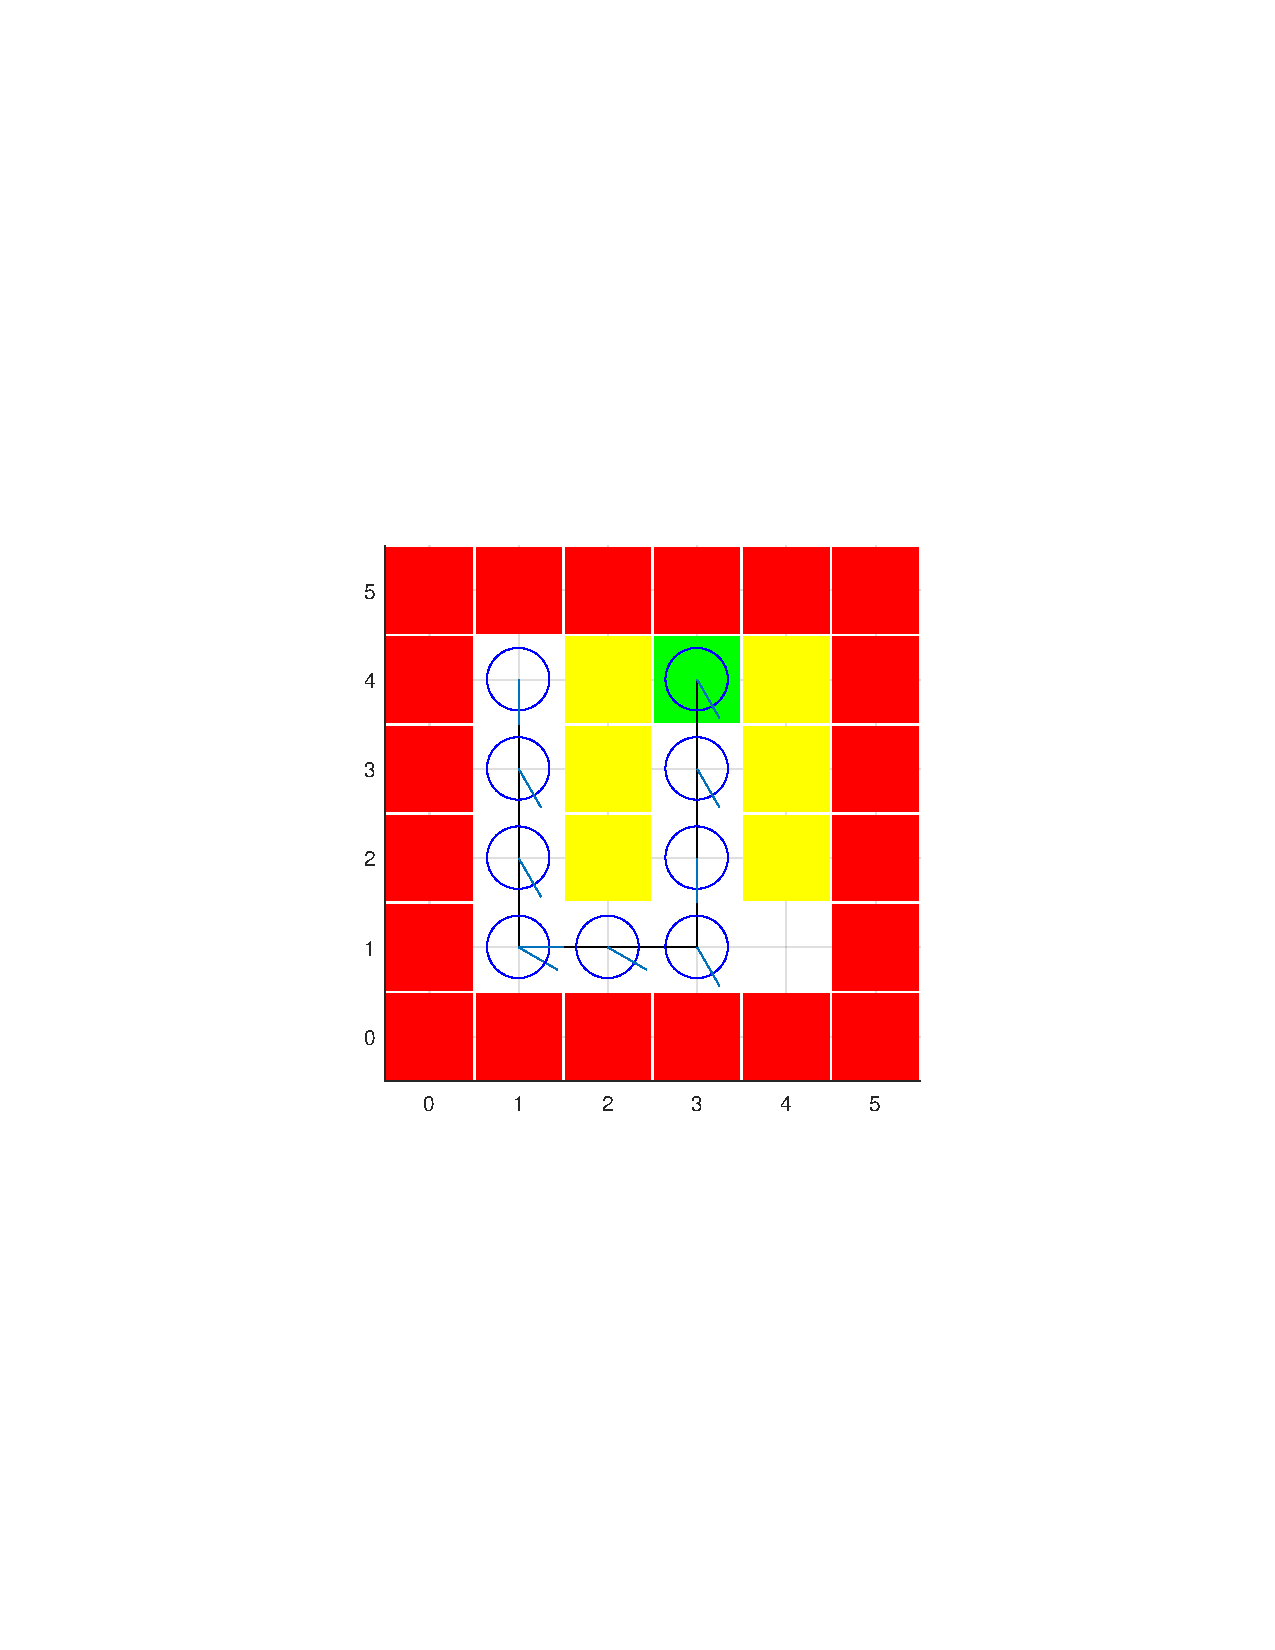
\includegraphics[trim={5cm 9cm 3cm 9cm},clip,scale = 0.7]{plots/Probabilistic/5bPe0.pdf}
				\label{fig:subfig2}} 
		\end{minipage}
		\qquad
		\begin{minipage}{0.4\textwidth}%
			\subfloat[Subfigure 2 list of figures text][Optimal Value ($V^*$)]{
				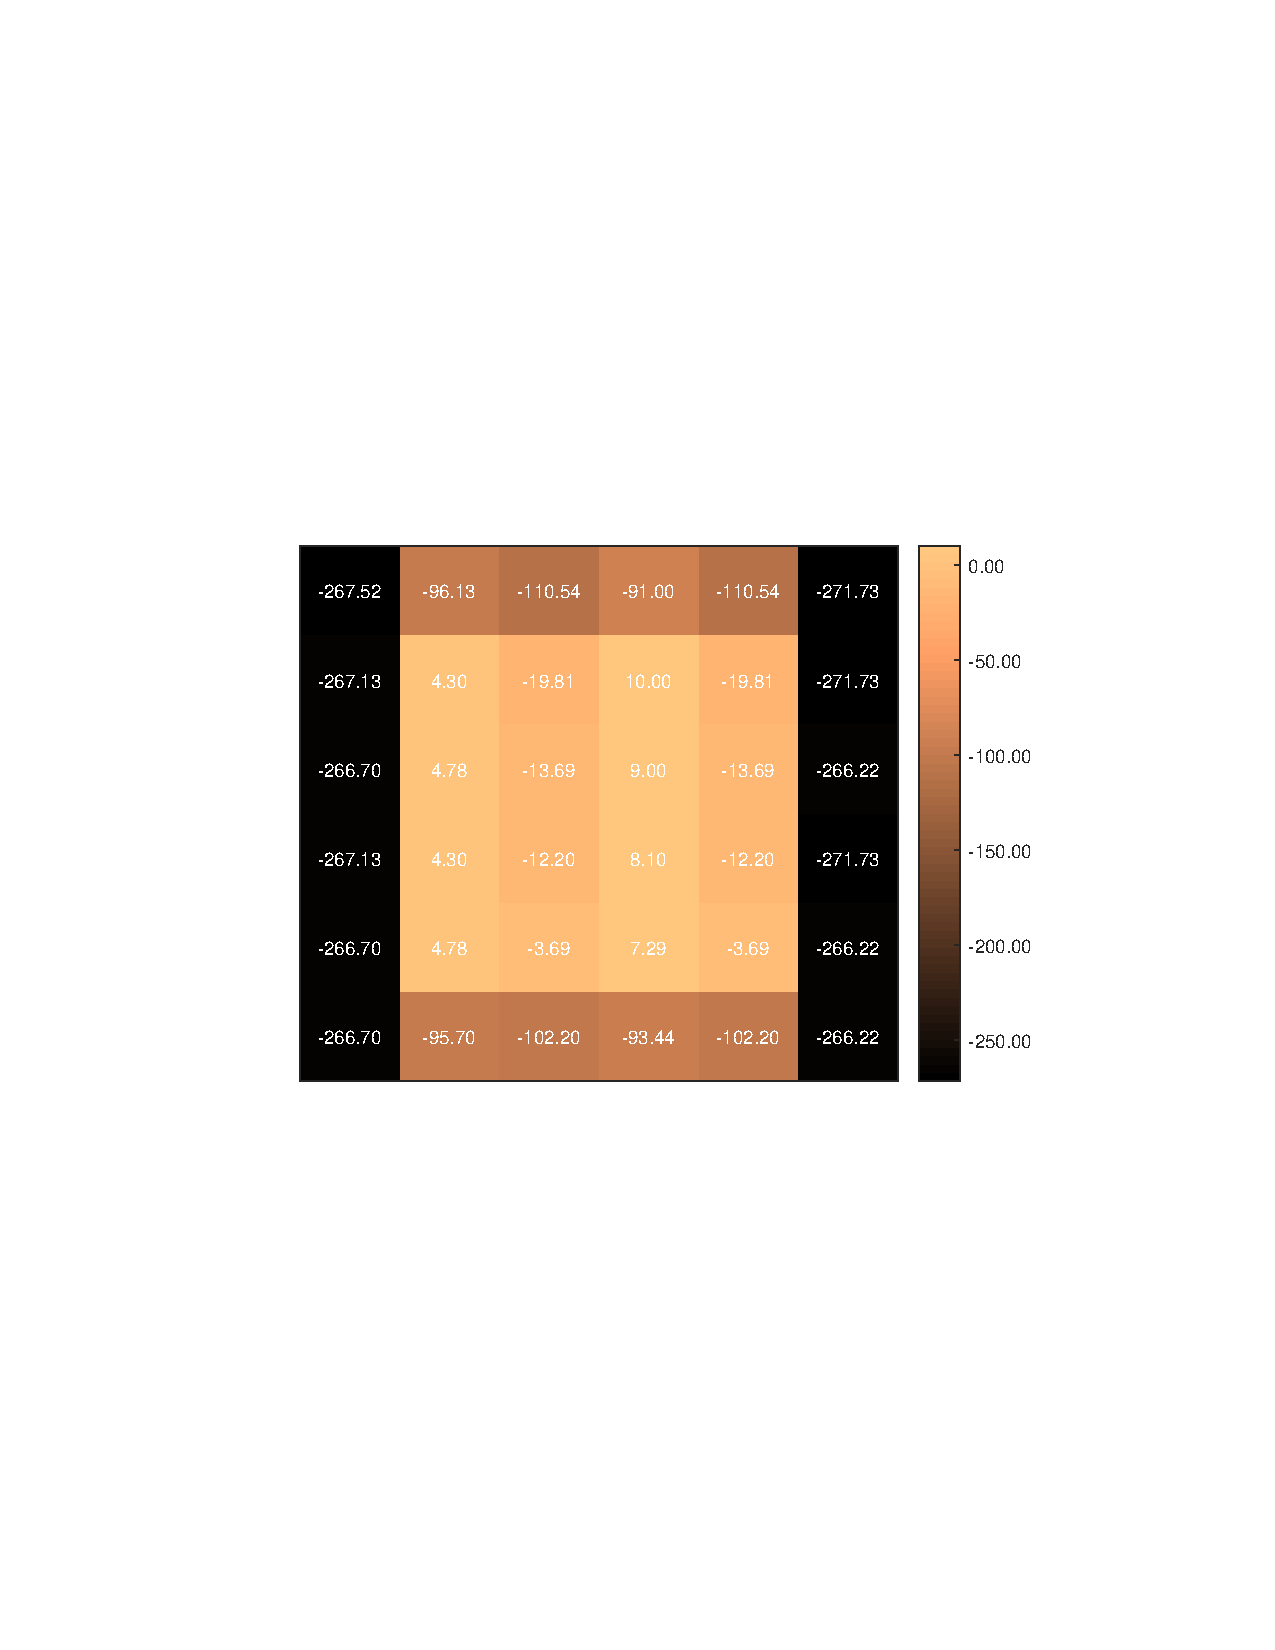
\includegraphics[trim={5cm 9cm 3cm 9cm},clip,scale = 0.7]{plots/Probabilistic/5bPe01.pdf}
				\label{fig:subfig2}} 
		\end{minipage}
		
		\caption{Question 5(b): $V^*$ and $P^*$ for limited heading +1 reward with $P_{e} = 0$ under value iteration.}
		\label{fig:globfig}
	\end{figure}


		\begin{figure}[h!]
	\centering
	\begin{minipage}{0.5\textwidth}%
		\subfloat[Subfigure 2 list of figures text][Optimal Policy ($P^*$)]{
			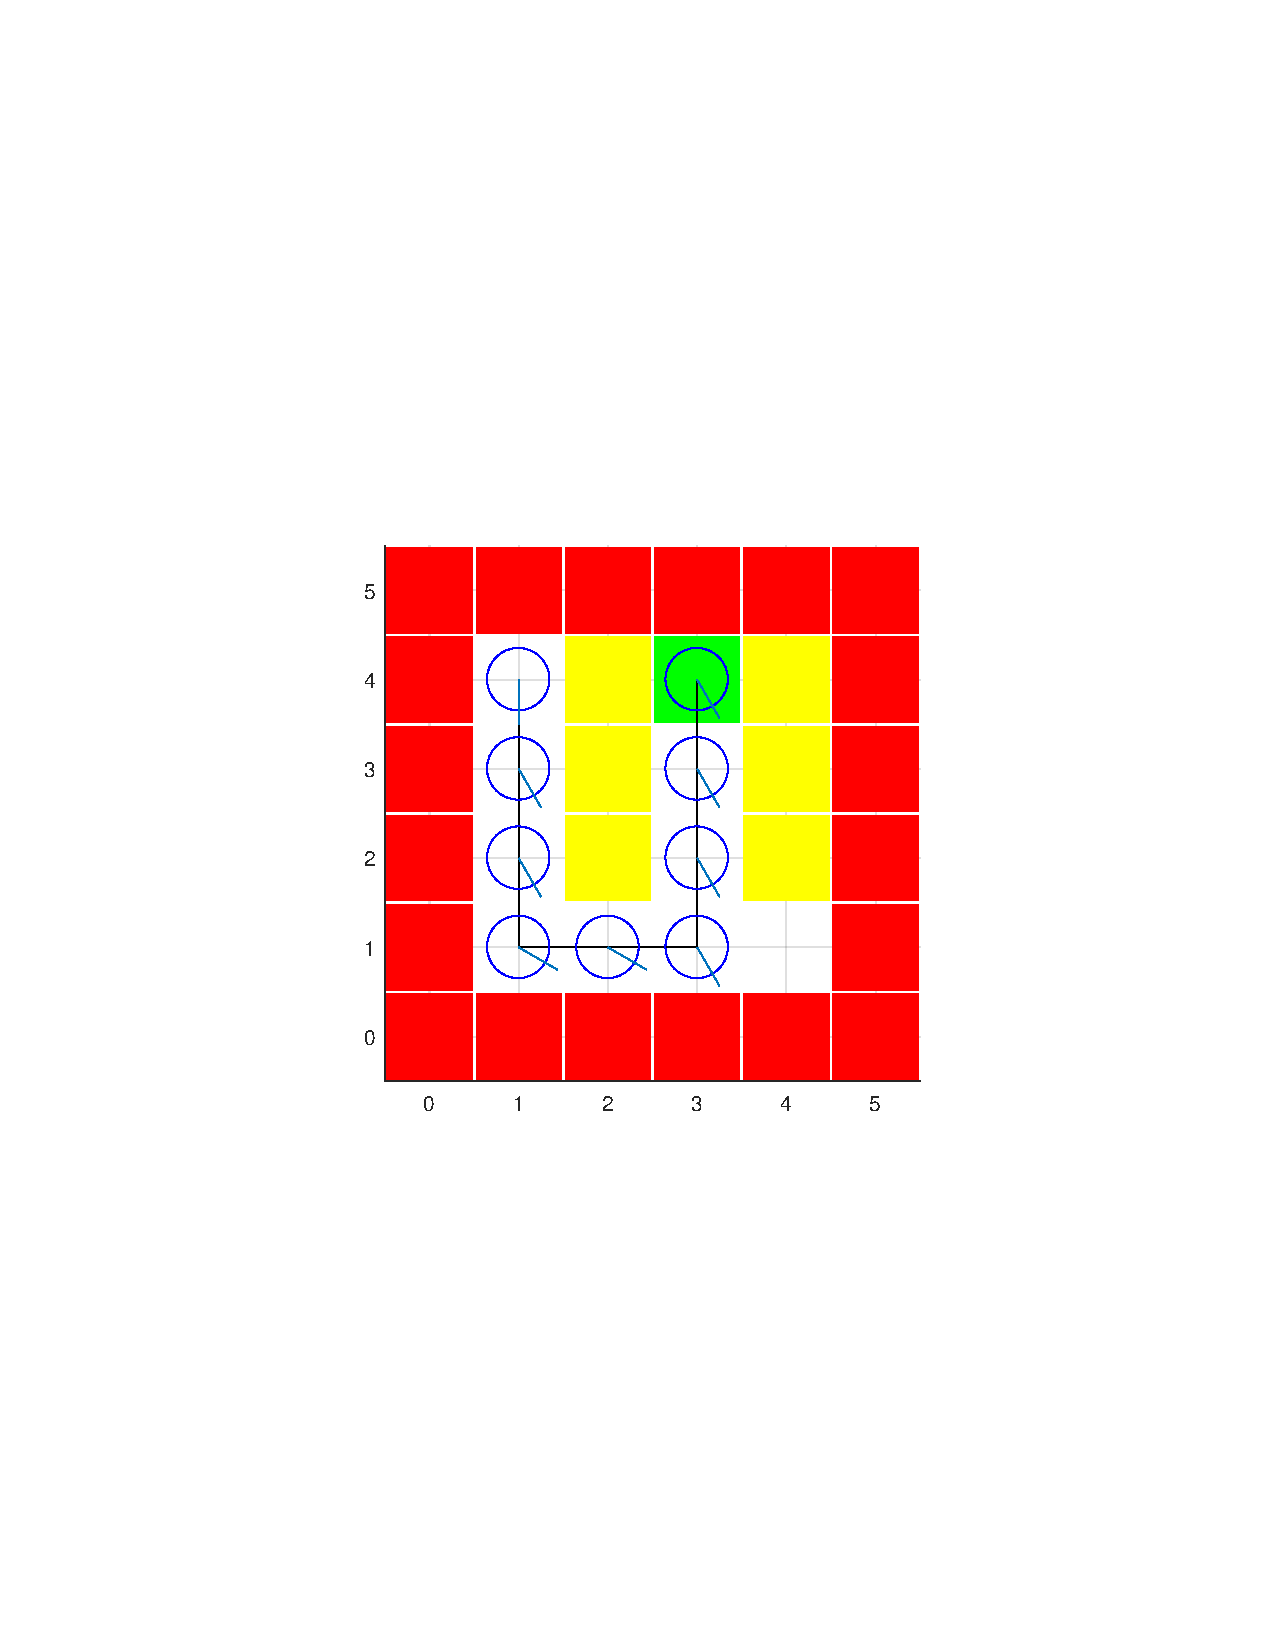
\includegraphics[trim={5cm 9cm 3cm 9cm},clip,scale = 0.7]{plots/Probabilistic/5bPe0PI_Traj.pdf}
			\label{fig:subfig2}} 
	\end{minipage}
	\qquad
	\begin{minipage}{0.4\textwidth}%
		\subfloat[Subfigure 2 list of figures text][Optimal Value ($V^*$)]{
			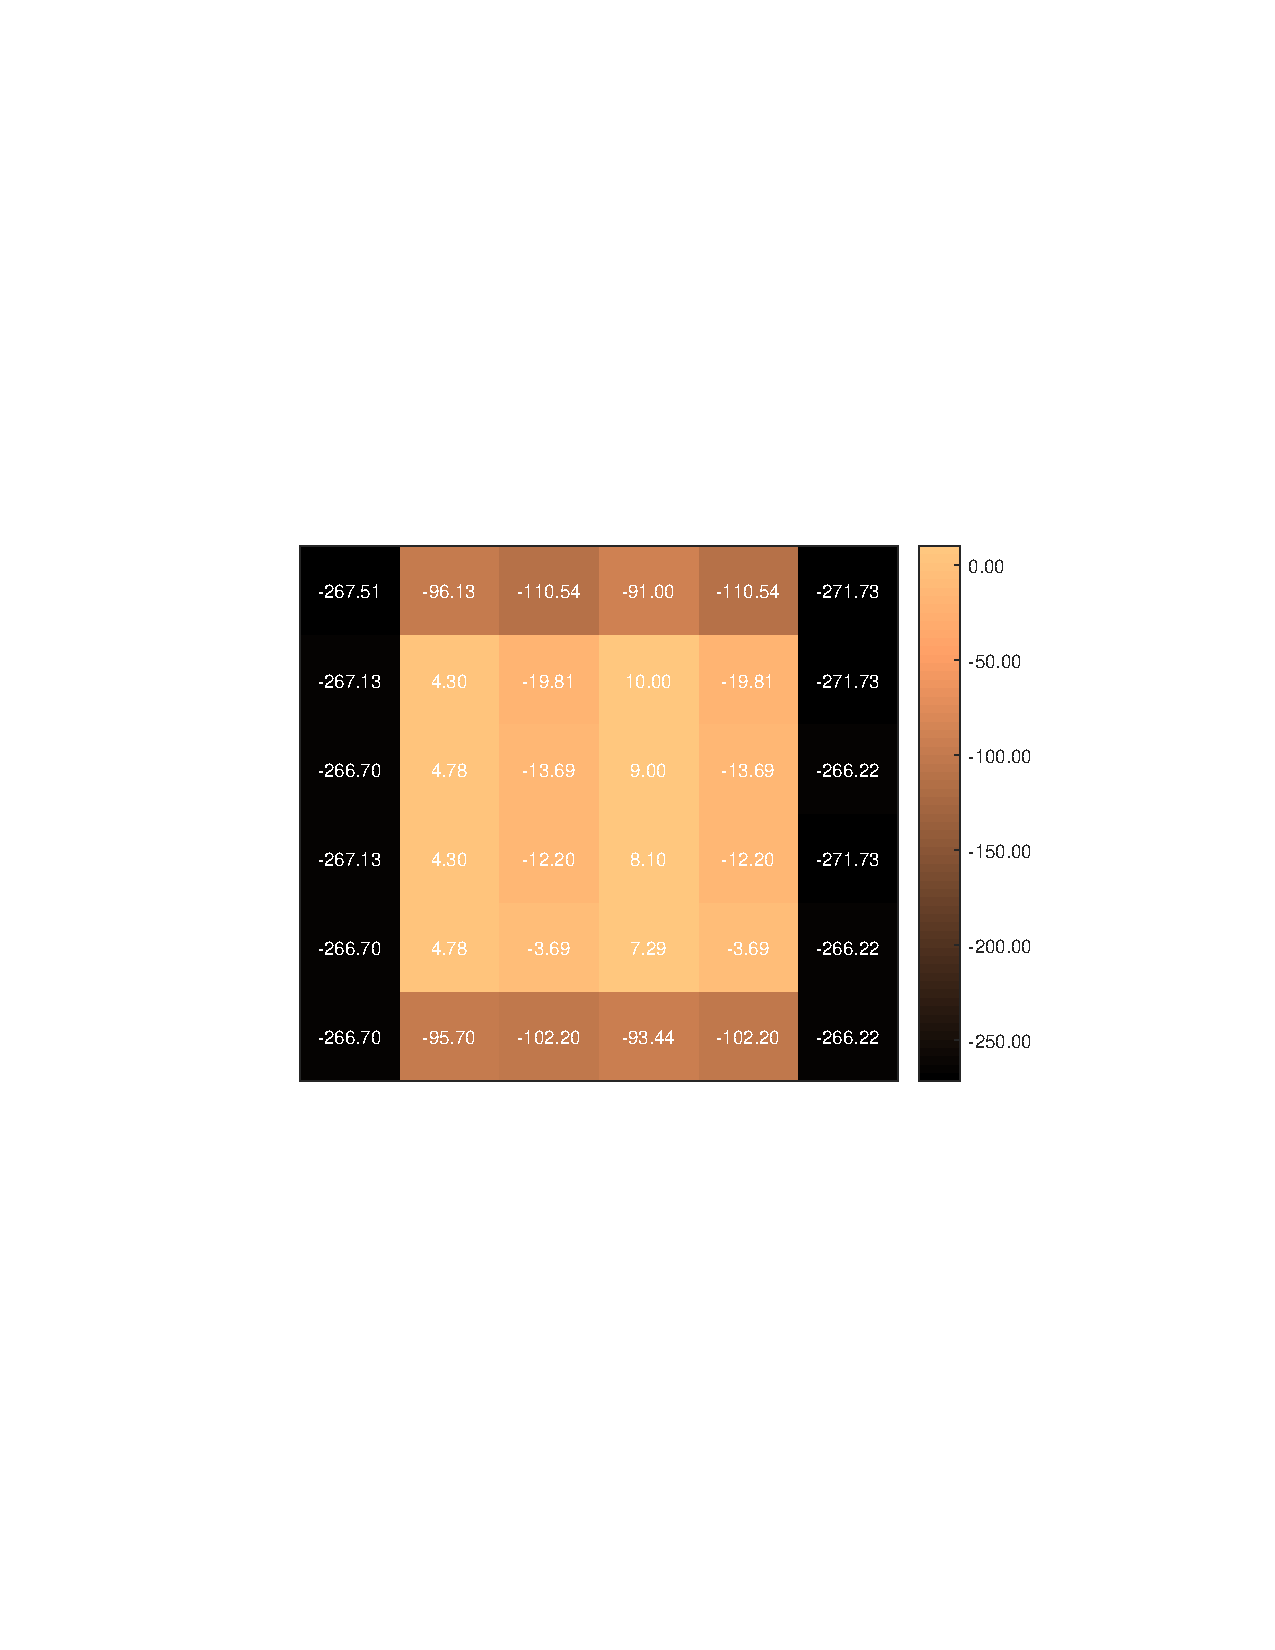
\includegraphics[trim={5cm 9cm 3cm 9cm},clip,scale = 0.7]{plots/Probabilistic/5bPe0PI_V.pdf}
			\label{fig:subfig2}} 
	\end{minipage}
	
	\caption{Question 5(b): $V^*$ and $P^*$ for limited heading +1 reward with $P_{e} = 0$ under policy iteration.}
	\label{fig:globfig}
\end{figure}

\vspace{50pt}  
\begin{figure}[h!]
	\centering
	\begin{minipage}{0.5\textwidth}%
		\subfloat[Subfigure 2 list of figures text][Expected Optimal Value ($V^*$) under $P_{e}=0.25$]{
			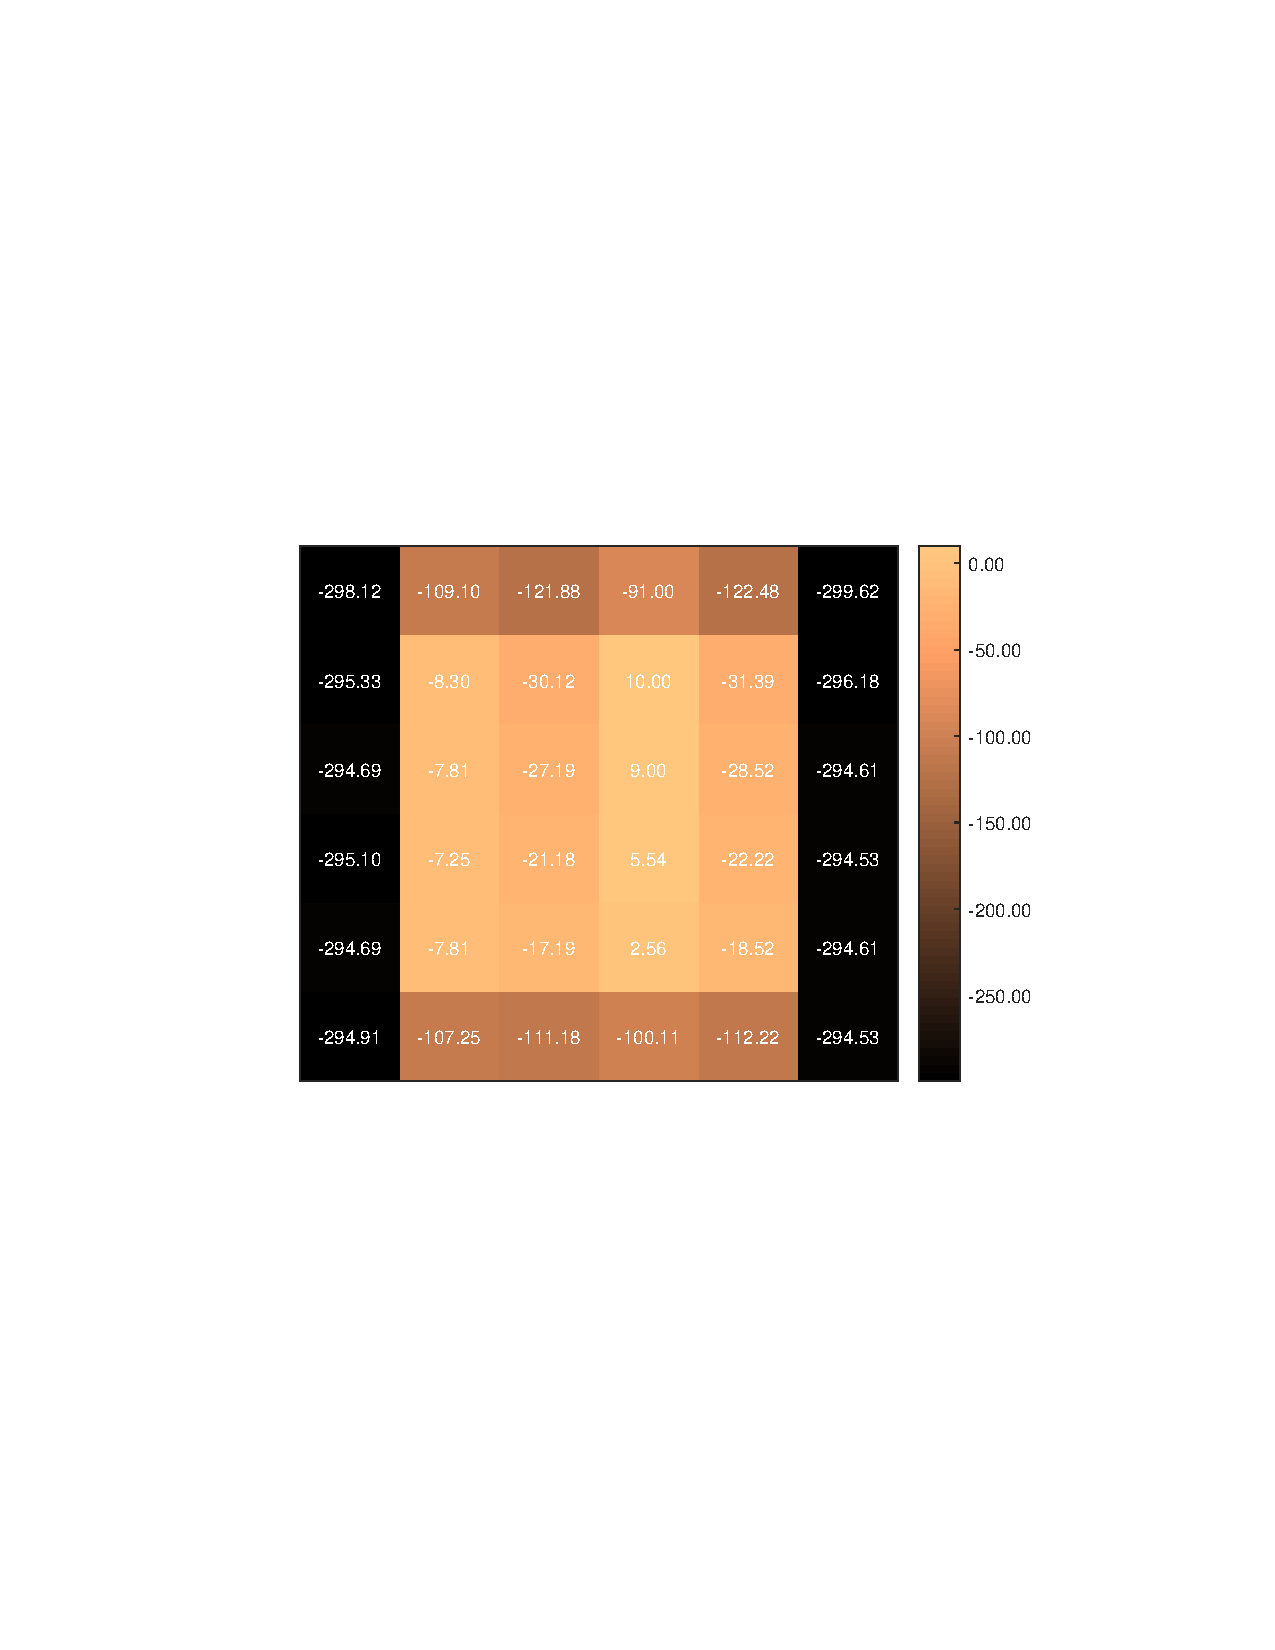
\includegraphics[trim={5cm 9cm 3cm 9cm},clip,scale = 0.55]{plots/Probabilistic/5b2.pdf}
			\label{fig:subfig2}} \\
		
		\subfloat[Subfigure 3 list of figures text][$V_{1}$ with value of 0.35]{
			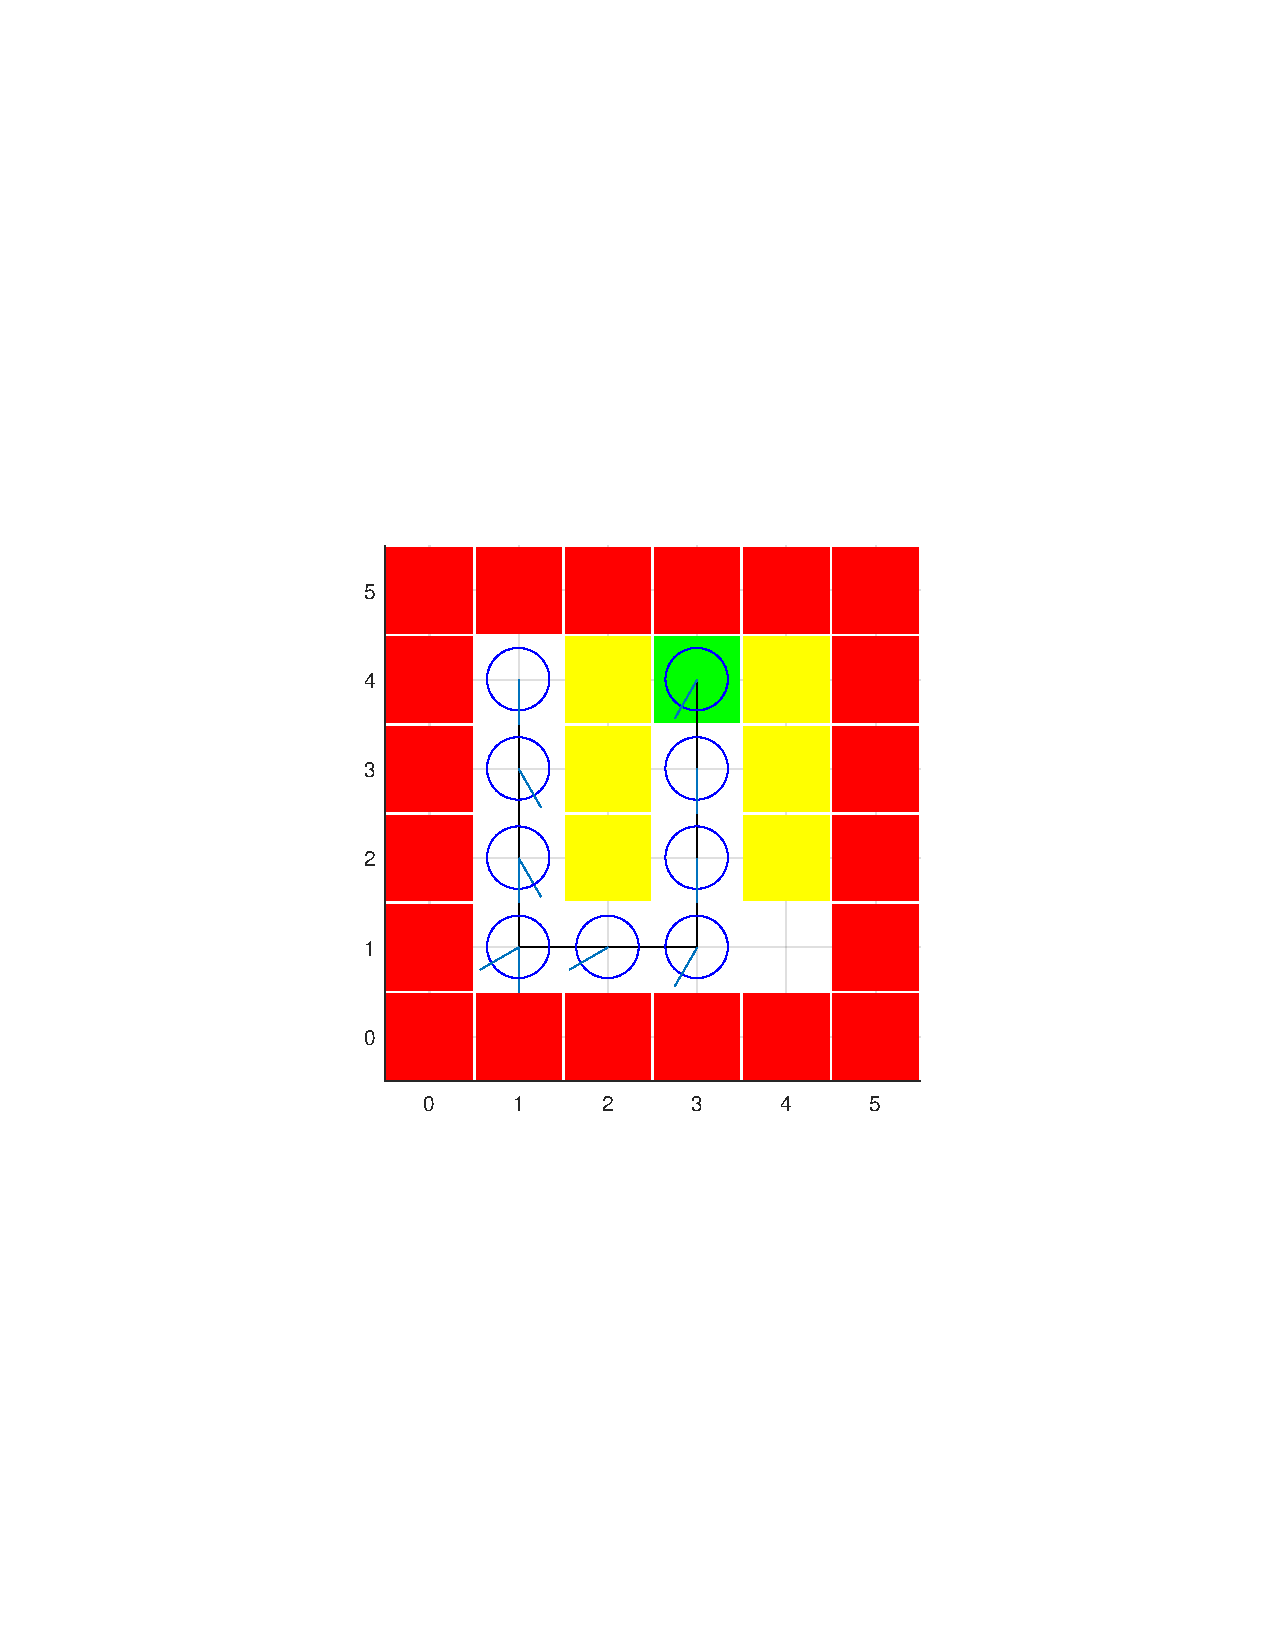
\includegraphics[trim={5cm 9cm 3cm 9cm},clip,scale = 0.55]{plots/Probabilistic/5b21.pdf}
			\label{fig:subfig2}} \\
		
		\subfloat[Subfigure 3 list of figures text][$V_{2}$ with value of -9.50]{
			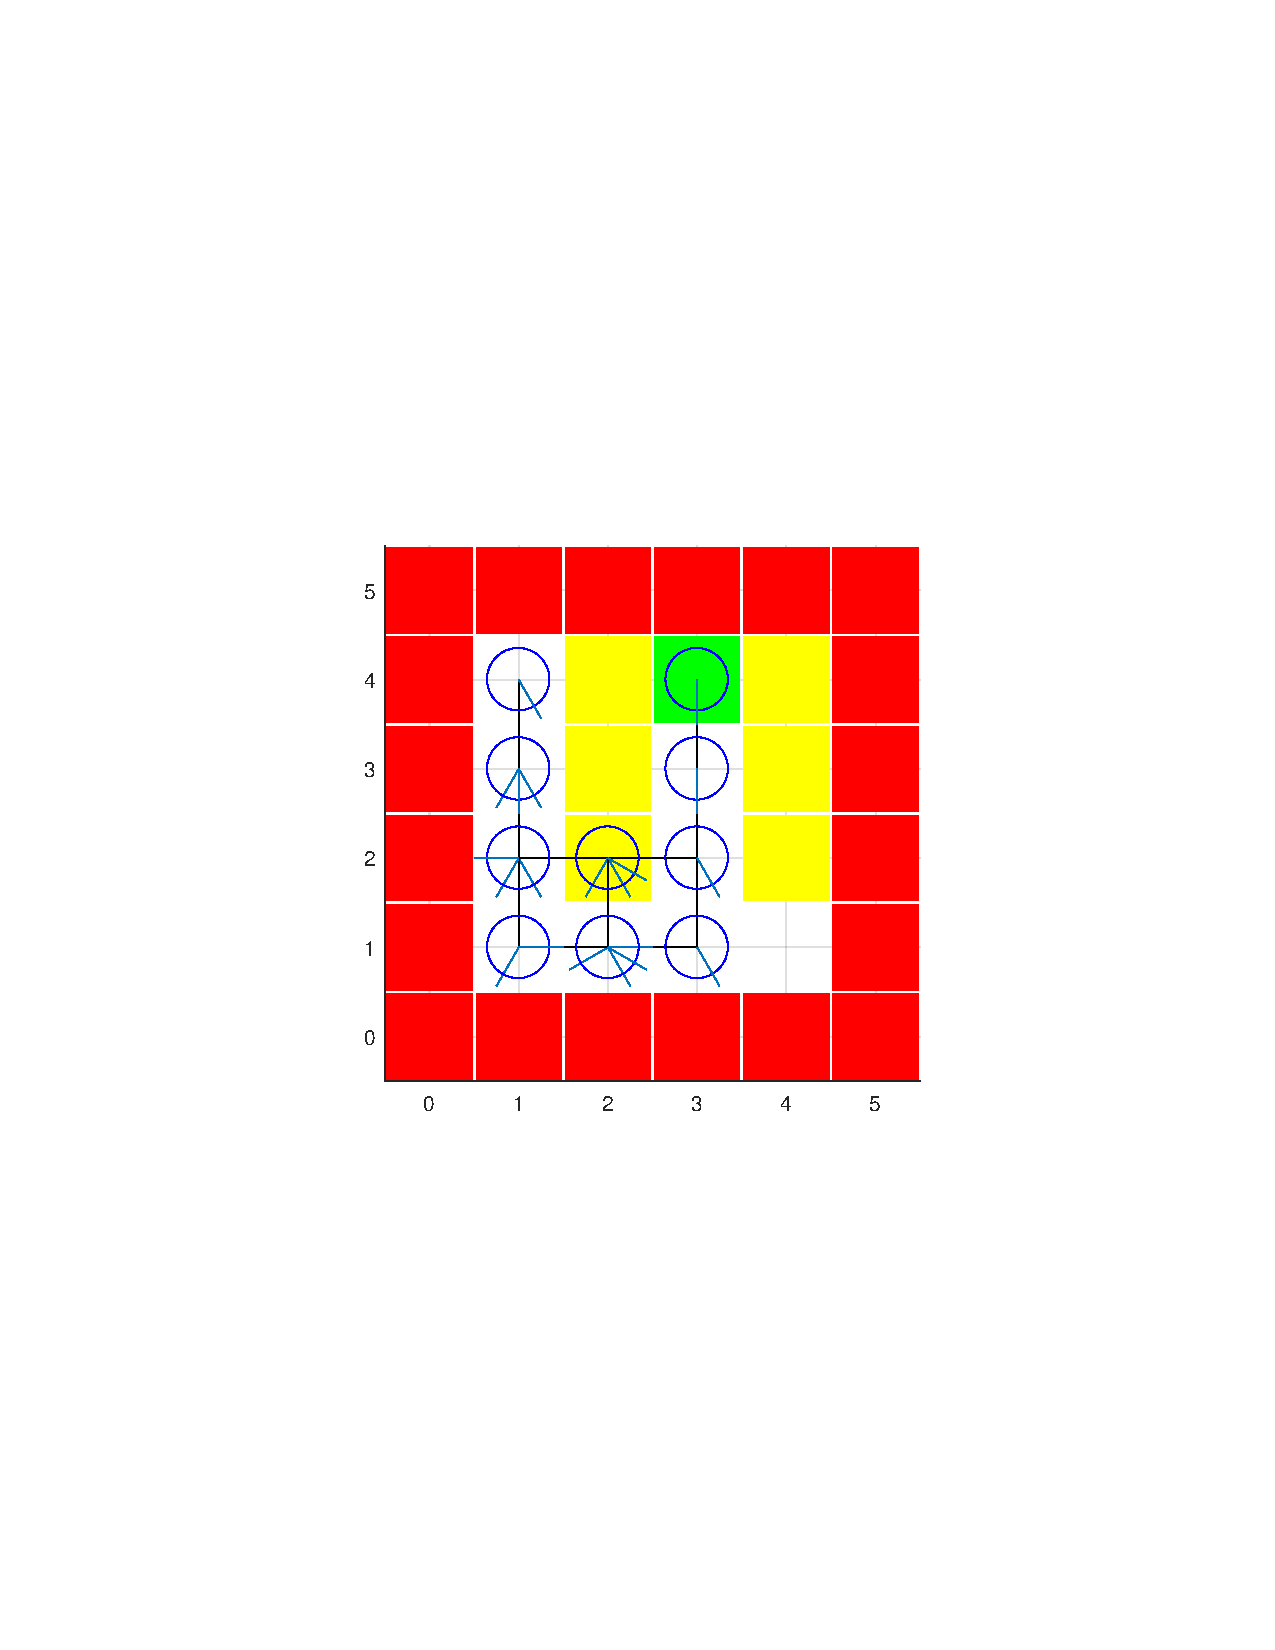
\includegraphics[trim={5cm 9cm 3cm 9cm},clip,scale = 0.55]{plots/Probabilistic/5b22.pdf}
			\label{fig:subfig2}} 
	\end{minipage}
	\qquad
	\begin{minipage}{0.4\textwidth}%
		\subfloat[Subfigure 2 list of figures text][$V_{3}$ with value of -16.24]{
			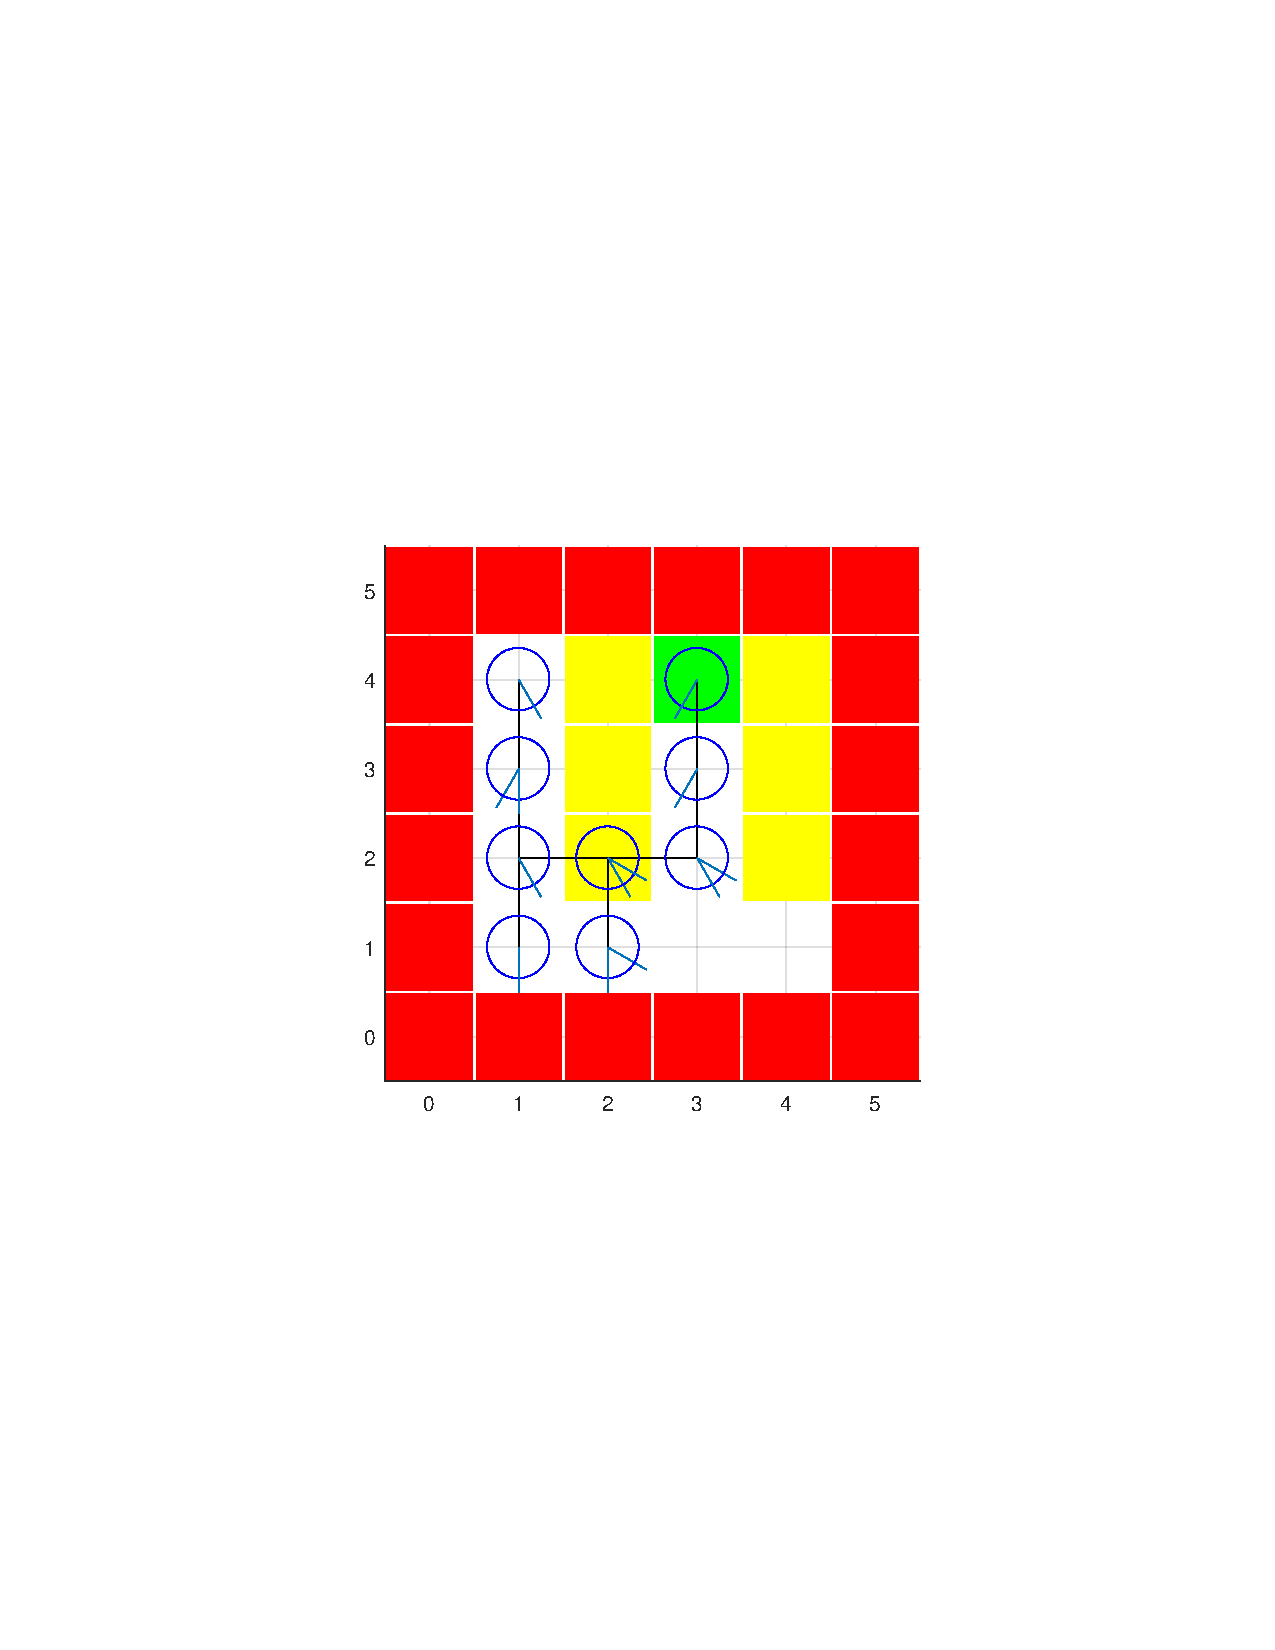
\includegraphics[trim={5cm 9cm 3cm 9cm},clip,scale = 0.55]{plots/Probabilistic/5b23.pdf}
			\label{fig:subfig2}} 
		
		\subfloat[Subfigure 3 list of figures text][$V_{4}$ with value of 0.23]{
			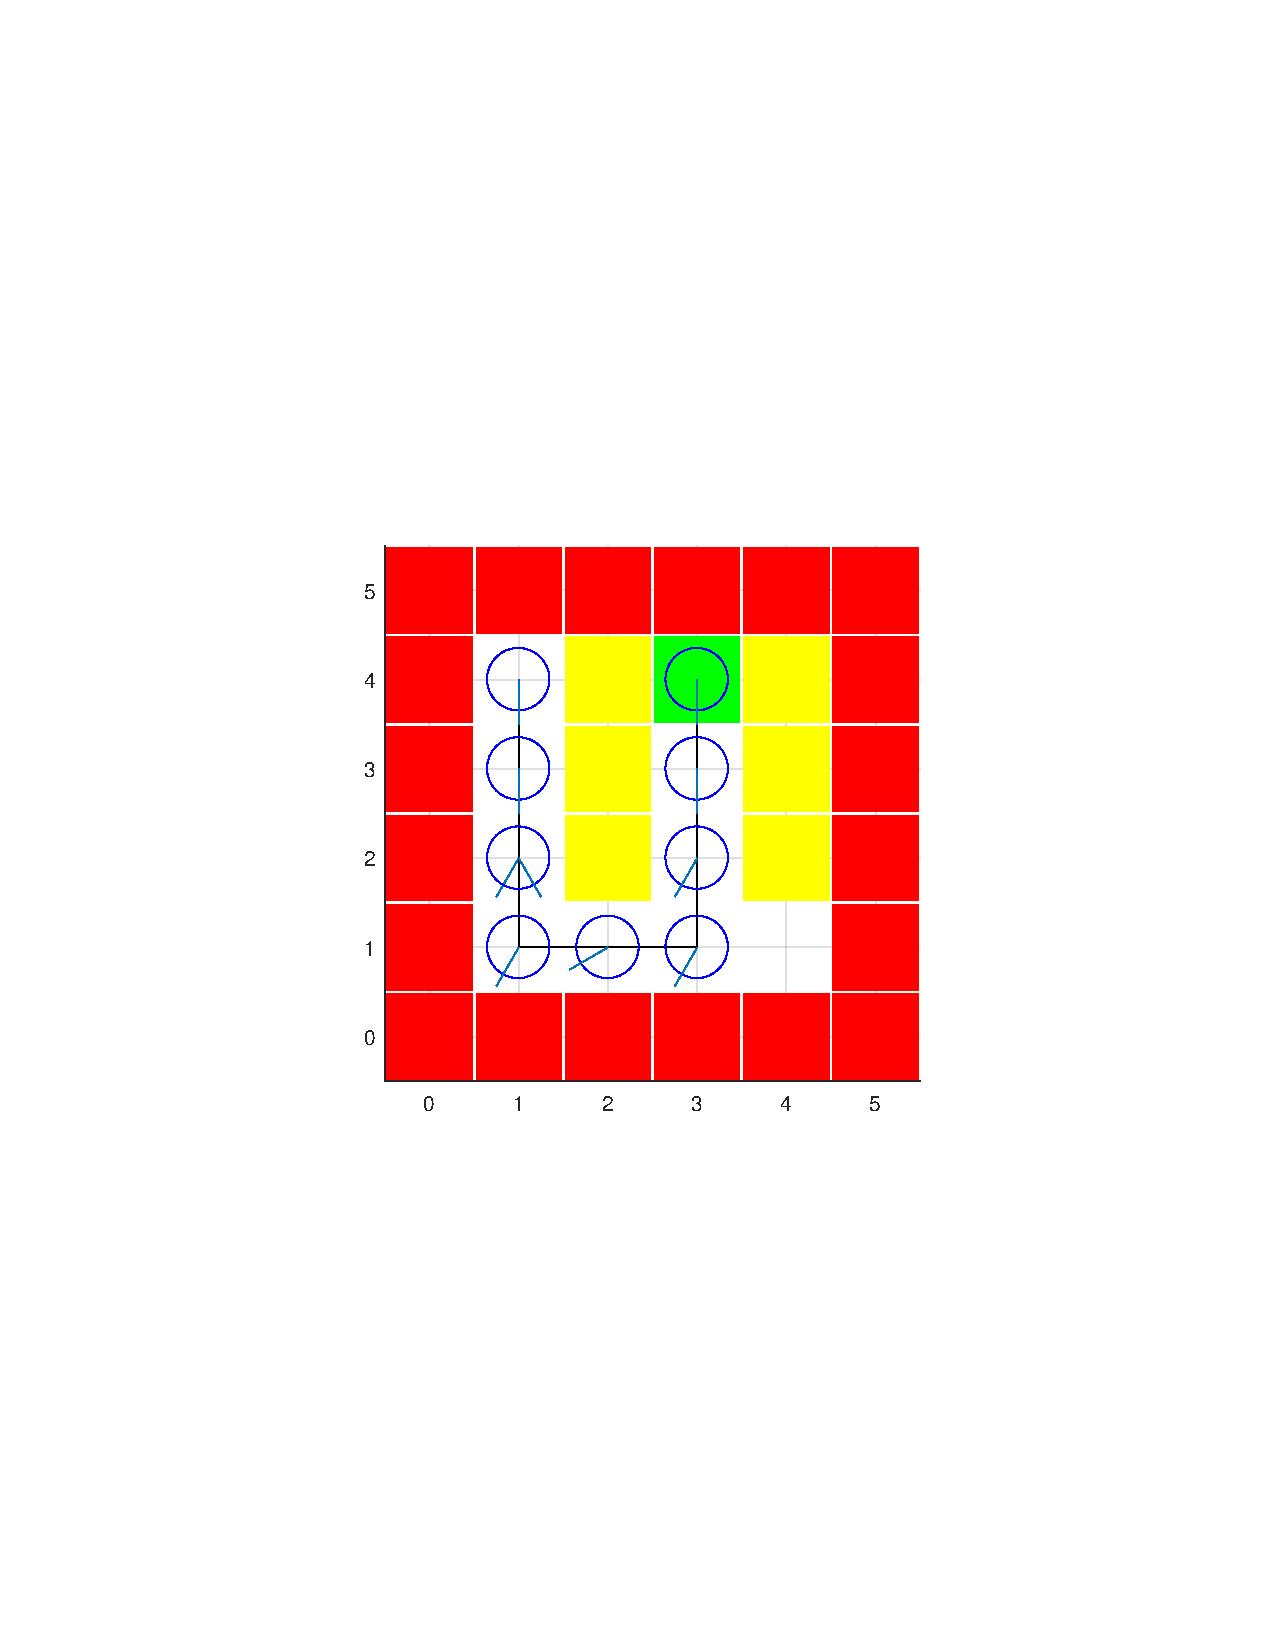
\includegraphics[trim={5cm 9cm 3cm 9cm},clip,scale = 0.55]{plots/Probabilistic/5b24.pdf}
			\label{fig:subfig3}} \\ 
		
		\subfloat[Subfigure 3 list of figures text][$V_{5}$ with value of -6.00]{
			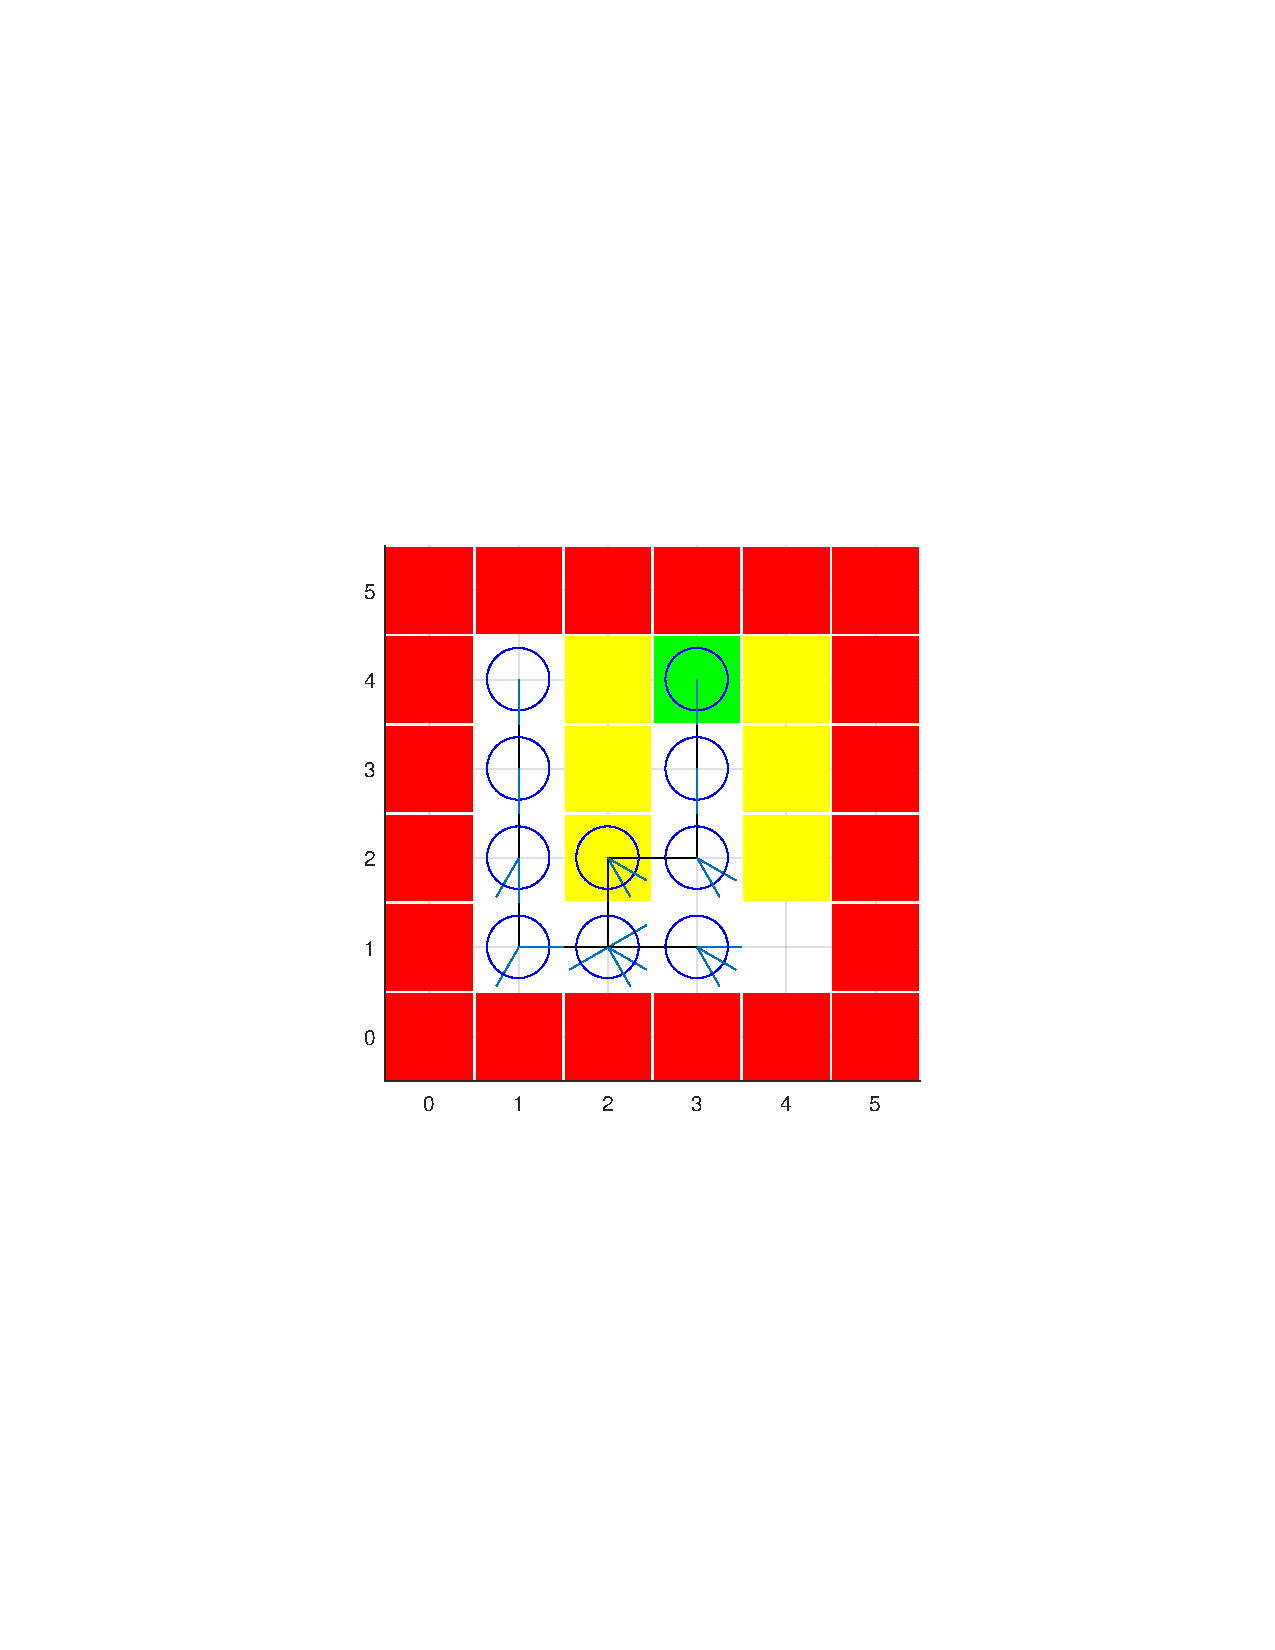
\includegraphics[trim={5cm 9cm 3cm 9cm},clip,scale = 0.55]{plots/Probabilistic/5b25.pdf}
			\label{fig:subfig3}} 
	\end{minipage}
	
	\caption{Question 5(b).}
	\label{fig:globfig}
\end{figure}	
	
	\newpage
	\noindent 5(c) 	The overal time that it took either policy and value iteration algorithms under different heading rewards and $p_{e}$ is shown in Table 1. It can be seen that the value iteration algorithm overall took longer compared to the policy iteration to converge. Also it can be seen that the limited heading reward took longer to converge than the one where heading does matter for the final reward. Also, it is witnessed that when $P_{e} = 0.25$ it took longer to converge for the algorithms compared to the $P_{e} = 0$. This is also expected since the uncertainty makes the robot to explore more on average which in turn makes the algorithm to converge slower.
	\begin{center}
		\begin{tabular}{ |c|c|c|c|c| } 
			\hline
			& All head. (Pr = 0) & All head. (Pr = 0.25) & limited head. (Pr = 0) & limited head. (Pr = 0.25) \\ \hline
			Policy iteration & 272 (s) & 373 (s) & 422 (s) & 477 (s) \\ \hline
			Value iteration & 571 (s) & 597 (s) & 705 (s) & 798(s) \\ \hline
			\hline
		\end{tabular}
			\captionof{table}{time to converge for value and policy iteration algorithms.} 
	\end{center}
	
	An interesting point for when $P_{e}$ was not zero is that for every realization of robot starting at (1,4,6), the trajectory of the robot will be different due to uncertainty from $P_{e}$ yet the $V^*$ and $P^*$ remain the same, since $V^*$ is in fact averages over all the possible realizations and not individual ones. This is different when $P_{e}$ is zero since for every realization of the system, the trajectory of the robot and V value for that trajectory remains the same. \\ 
	
	When one of the actions that robot can take is to stay still and do nothing, then for some robot trajectories where it needs to pass through those states the robot will stay and cannot hit the goal. Two options at least are available. One is to put some limits on the number of iterations for either value iteration or policy iteration so that if robot did not converge the program will be terminated. In my opinion this is kind of not nice/realistic given the fact that our robot does want to hit the goal and also has other actions to take. The second option is that whenever the optimum policy was to stay still, we do not pick that and find second best action that would maximize the Bellman equation. This is nice since at least staying still would not some how break the program and the robot will hit the goal. \\
	
	Another interesting point here was that even though both the policy and value iteration algorithms converge to the same $V^*$, they did not converge to the same optimal policy. This should not be surprising as they solve the same Bellman equation for $V^*$ but it was witnessed that actually different policies can acheive the same $V^*$ values which was an interesting point to learn from this homework.\\ 
	
	Another observation is that under some initial conditions and some policies for when $P_{e} = 0$, the robot would not converge to the goal, for example it could infinitely switch back and forth between two states. This brings up the point that in general this can happen with some specific MDPs. In fact the question is what happens when the agent bounces between two or more states where the actions some states would cancel out the actions in other states and make the agent not able to skip some inner manifolds within the state space. So in this case we would have that the robot would not converge. As a result what I think happens is that in fact having some sort of uncertainty into our dynamics ($P_{e}$ here) improves the overal convergence behavior of the robot. This is somehow helps the robot to escape the local minimum or some lower dimention optimal manifold within the robot's state space. I believe very similar underlying idea is used for methods like stochastic gradient decent where uncertainty improves escaping unwanted local minimums. 

\end{document}